\documentclass[11pt,a4paper]{article}

\usepackage[margin=2.3cm]{geometry}
\usepackage{amsmath,amssymb}
\usepackage{booktabs}
\usepackage{xcolor}
\usepackage[colorlinks=true,linkcolor=blue!50!black,urlcolor=blue!55!black]{hyperref}
\usepackage{tcolorbox}
\usepackage{enumitem}
\usepackage{titlesec}
\usepackage{tikz}
\usetikzlibrary{arrows.meta}
\usepackage{placeins}
\usepackage{bm}
\usepackage{algorithm}
\usepackage{algpseudocode}

\titleformat{\section}{\normalfont\Large\bfseries\color{blue!45!black}}{\thesection}{1em}{}
\newcommand{\code}[1]{\texttt{\small #1}}

% Figures and every count quoted below are generated from the mesh connectivity by
% python/cvfem_locality_figures.py; nothing here assumes a stencil.
%% generated by python/cvfem_locality_figures.py
\newcommand{\nbr}{$E_1$}
\newcommand{\ncoarseCrossExactEdge}{1}
\newcommand{\ncoarseCrossExactInt}{5}
\newcommand{\ncoarseCrossFrozenEdge}{0}
\newcommand{\ncoarseCrossFrozenInt}{0}
\newcommand{\ncoarseExactEdge}{16}
\newcommand{\ncoarseExactInt}{14}
\newcommand{\ncoarseFrozenEdge}{9}
\newcommand{\ncoarseFrozenInt}{9}
\newcommand{\ncrossCorner}{5}
\newcommand{\ncrossInt}{0}
\newcommand{\ncrossNear}{3}
\newcommand{\nexactCorner}{20}
\newcommand{\nexactInt}{21}
\newcommand{\nexactNear}{21}
\newcommand{\nfrozenCorner}{9}
\newcommand{\nfrozenInt}{9}
\newcommand{\nfrozenNear}{9}
\newcommand{\ngradEdge}{9}
\newcommand{\ngradEdgeCells}{4}
\newcommand{\nkNear}{5}
\newcommand{\npathCellsN}{4}
\newcommand{\npathCellsNM}{2}
\newcommand{\nquadCrossCorner}{11}
\newcommand{\nquadCrossFrozen}{0}
\newcommand{\nquadCrossInt}{12}
\newcommand{\nquadRowCorner}{20}
\newcommand{\nquadRowFrozen}{9}
\newcommand{\nquadRowInt}{21}
\newcommand{\nregThreeCoarseExact}{81}
\newcommand{\nregThreeCoarseFrozen}{27}
\newcommand{\nregThreeExact}{81}
\newcommand{\nregThreeFrozen}{27}
\newcommand{\nregTwoCoarseExact}{21}
\newcommand{\nregTwoCoarseFrozen}{9}
\newcommand{\nregTwoExact}{21}
\newcommand{\nregTwoFrozen}{9}


\definecolor{ink}{HTML}{1D2330}
\definecolor{meshgrey}{HTML}{B4BAC6}
\definecolor{dualgrey}{HTML}{7F8AA0}
\definecolor{localblue}{HTML}{2166AC}
\definecolor{crossred}{HTML}{C8452B}
\definecolor{gradamber}{HTML}{B7791F}
\definecolor{facegreen}{HTML}{1B7F79}
\definecolor{cvtint}{HTML}{DCE8F4}
\definecolor{celltint}{HTML}{E8E8E5}
\definecolor{gradtint}{HTML}{F6E3BF}

\tikzset{
  micro/.style={draw=meshgrey, line width=0.35pt},
  microfaint/.style={draw=meshgrey!55, line width=0.3pt},
  coarse/.style={draw=dualgrey, line width=0.7pt},
  macro/.style={draw=ink, line width=1.3pt, line join=round},
  element/.style={draw=ink!70, line width=0.55pt, line join=round},
  % Elements are drawn solid and tinted neutral grey; control volumes, their dual, are dotted
  % and tinted blue -- the same blue as V_i in the formulas.
  dual/.style={draw=localblue!50, line width=0.4pt, dash pattern=on 0.6pt off 1.1pt, line cap=round},
  cvline/.style={draw=localblue!80, line width=0.75pt, dash pattern=on 0.9pt off 1.2pt, line cap=round},
  elemlabel/.style={font=\scriptsize, text=ink!80, inner sep=0.5pt},
  cvlabel/.style={font=\scriptsize, text=localblue, inner sep=0.5pt},
  cvfill/.style={fill=cvtint},
  cellfill/.style={fill=celltint},
  gradfill/.style={fill=gradtint},
  gradstrong/.style={fill=gradamber!45},
  dvec/.style={draw=ink, line width=0.8pt, -{stealth[length=4pt]}},
  avec/.style={draw=facegreen, line width=0.9pt, -{stealth[length=4pt]}},
  kpath/.style={draw=facegreen, line width=1.4pt, -{stealth[length=6pt]}},
  gpath/.style={draw=gradamber, line width=1.4pt, dash pattern=on 3pt off 1.5pt, -{stealth[length=6pt]}},
  nodelabel/.style={font=\footnotesize, text=ink, fill=white, fill opacity=0.8, text opacity=1, inner sep=1pt},
  kface/.style={draw=facegreen, line width=1.3pt},
  reach/.style={circle, fill=localblue, inner sep=0pt, minimum size=3.8pt},
  cross/.style={circle, fill=crossred, inner sep=0pt, minimum size=4.4pt},
  reachc/.style={circle, fill=localblue, inner sep=0pt, minimum size=5.4pt},
  crossc/.style={circle, fill=crossred, inner sep=0pt, minimum size=5.4pt},
  support/.style={circle, fill=meshgrey, inner sep=0pt, minimum size=2.6pt},
  gradnode/.style={rectangle, draw=gradamber, fill=gradamber!25, line width=0.9pt, inner sep=0pt, minimum size=5.2pt},
  gradring/.style={rectangle, draw=gradamber, line width=0.9pt, inner sep=0pt, minimum size=6.4pt},
  rownode/.style={circle, draw=ink, fill=white, line width=1.1pt, inner sep=0pt, minimum size=6pt},
  macrolabel/.style={font=\small\itshape, text=ink, fill=white, fill opacity=0.85, text opacity=1, inner sep=1pt},
  note/.style={font=\scriptsize, text=ink, fill=white, inner sep=1pt},
  notedot/.style={circle, draw=ink, line width=0.8pt, inner sep=0pt, minimum size=4pt},
  panel/.style={font=\footnotesize, text=ink, inner sep=0pt},
}
% The figures' colour roles, for the formulas: green faces and K, amber gradients, G and W,
% blue control volumes and A_frozen, red nodes no macro-element shares with the row's node.
\newcommand{\cf}[1]{{\color{facegreen}#1}}
\newcommand{\cg}[1]{{\color{gradamber}#1}}
\newcommand{\cv}[1]{{\color{localblue}#1}}
\newcommand{\cx}[1]{{\color{crossred}#1}}
% Robust: these sit inside captions, which expand their argument.
\DeclareRobustCommand{\key}[1]{\tikz[baseline=-0.6ex]\node[#1] {};}
\DeclareRobustCommand{\keyline}[1]{\tikz[baseline=-0.6ex]\draw[#1] (0,0) -- (0.35,0);}

\title{\bfseries Where the CVFEM operators reach\\
\large Exactness, macro-element locality and the coarse space, drawn in two dimensions}
\date{\today}

\begin{document}
\maketitle

\begin{tcolorbox}[colback=blue!4,colframe=blue!50!black,title={\bfseries Two different properties}]
\textbf{Exact} is a statement about \emph{which terms} an operator contains. The Jacobian is
\[
J_{\text{exact}} \;=\; \cv{A_{\text{frozen}}} \;+\; \cf{K}\,\cg{W^{-1}G} .
\]
The matrix-free Jacobian that FGMRES and Newton apply contains both terms, at every node. The
assembled operators --- the Galerkin coarse levels and the Vanka patches --- contain
$A_{\text{frozen}}$ at every node and $K W^{-1} G$ at none.

\textbf{Macro-element local} is a statement about \emph{which node pairs} a term couples. The
element-wise assembly stores a sum of macro-element matrices, so it can hold an entry $(i,m)$
only if some macro-element contains both $i$ and $m$. Every entry of $A_{\text{frozen}}$
satisfies that. Some entries of $K W^{-1} G$ do not, and those are the ones drawn in red below.
\end{tcolorbox}

\section{The mesh}

The semi-structured mesh is an unstructured mesh of macro-elements, each refined uniformly.
Figure~\ref{fig:mesh} is the two-dimensional analogue used throughout: a triangle tiled by three
quadrilateral macro-elements $E_0, E_1, E_2$ meeting at a vertex of valence three --- a vertex no structured
grid has --- each refined into $4\times4$ micro-cells. Inside one macro-element the nodes form a
lattice; across macro-elements they are shared through global node ids, and neighbouring
lattices are oriented differently. Every set drawn in this note is computed from that
connectivity, through global ids, by \code{python/cvfem\_locality\_figures.py}.

\begin{figure}[h]
\centering
\input{figures/locality_mesh.tex}
\caption{Two meshes on one set of nodes. The \emph{elements} are the micro-cells
(\keyline{micro}, one tinted grey, $\Omega_c$): the finite-element shape functions, gradients and
cell areas live on them, and they tile each macro-element (thick). The \emph{control volumes}
are their dual (\keyline{dual}, one tinted blue, $\cv{V_i}$): one around each node, bounded by
sub-control-volume faces that run from an element's centre to its edge midpoints. The balance
equations are integrated over control volumes; every face $\cf{s}$ \keyline{kface} of $\cv{V_i}$
lies inside one element and separates $i$ \key{rownode} from one edge neighbour. The circled
vertex is shared by three macro-elements.}
\label{fig:mesh}
\end{figure}

\section{The three factors}

\subsection{The formulas, on the drawing}

Every quantity below has a place in Figure~\ref{fig:anatomy}, and the formulas use the figure's
colours: \cf{green} for faces and $\cf{K}$, \cg{amber} for gradients, $\cg{G}$ and $\cg{W}$,
\cv{blue} for the control volume and $\cv{A_{\text{frozen}}}$, and \cx{red} for a node that no
macro-element shares with $i$. Two meshes share the nodes: the \emph{elements} $\Omega_c$ (the
micro-cells, solid edges, tinted grey), which carry the shape functions $N_a$ and every gradient,
and the \emph{control volumes} $\cv{V_i}$ (dotted blue edges, tinted blue), one per node, over
which the equations are balanced. Node $i$ owns $\cv{V_i}$. Inside an element $\Omega_c$, the
boundary of $\cv{V_i}$ consists of two sub-control-volume faces \keyline{kface}, each running
from the element centre to the midpoint of an edge $(i,j)$. A face
$\cf{s}$ carries an area vector $\cf{\bm a_s}$ and the edge vector $\bm d_s = \bm x_j - \bm x_i$
(both drawn in panel a). $\sigma_{is}=\pm1$ orients face $\cf{s}$ out of $\cv{V_i}$.

\paragraph{The residual.} The mass flux through face $\cf{s}$ is the averaged velocity flux minus
the Rhie--Chow correction,
\begin{equation}
\cf{\dot m_s} \;=\; \rho\,\bar{\bm u}_s\cdot\cf{\bm a_s} \;-\; c_s\Big[(p_j-p_i) - \tfrac12\,(\cg{\bm g_i+\bm g_j})\cdot\bm d_s\Big],
\label{eq:mdot}
\end{equation}
and the continuity residual of node $i$ sums it over the faces of $\cv{V_i}$,
$R^p_i = \sum_{\cf{s}\in\partial \cv{V_i}}\sigma_{is}\,\cf{\dot m_s}$. Here $\cg{\bm g_n}$ is the
reconstructed nodal pressure gradient: the gradients of the micro-cells around $\cg{n}$ (shaded
amber in panel b), weighted by their areas,
\begin{equation}
\cg{\bm g_n} \;=\; \frac{1}{\cg{W_n}}\sum_{c\ni n} |\Omega_c|\,\nabla p\big|_c,
\qquad
\cg{W_n} = \sum_{c\ni n}|\Omega_c|,
\qquad
\nabla p\big|_c = \sum_{a\in c} p_a\,\nabla N_a\big|_c .
\label{eq:grad}
\end{equation}

\paragraph{The Jacobian.} Differentiating~\eqref{eq:mdot} in a pressure direction $\delta p$
gives two groups of terms:
\begin{equation}
\delta R^p_i \;=\;
\cv{\underbrace{\sum_{s\in\partial V_i}\sigma_{is}\,c_s\,(\delta p_i-\delta p_j)}_{A_{\text{frozen}}:\ \text{nodes } i,j \text{ of one element}}}
\;+\;
\underbrace{\sum_{\cf{s}\in\partial V_i}\cf{\sigma_{is}\,\tfrac12\,c_s\,\bm d_s}\cdot(\cg{\delta\bm g_i+\delta\bm g_j})}_{\cf{K}\,\cg{W^{-1}G}:\ \text{through } \cg{\delta\bm g}}.
\label{eq:jac}
\end{equation}
The first group, together with the velocity columns, is $\cv{A_{\text{frozen}}}$: every term of
face $s$ reads only the corners of the element that contains $s$ (panel a). The second group is where
the gradient enters, and by~\eqref{eq:grad} $\cg{\delta\bm g_n}$ is linear in $\delta p$. Written
as matrices,
\begin{equation}
\cg{[G]_{nm}} = \cg{\sum_{c\ni n,\;c\ni m} |\Omega_c|\,\nabla N_m\big|_c},
\qquad
\cg{[W]_{nn}} = \cg{W_n},
\qquad
\cf{[K]_{in}} = \cf{\sum_{\substack{s\in\partial V_i\\ n\in\{i,\,j_s\}}} \tfrac12\,\sigma_{is}\,c_s\,\bm d_s^{\mathsf T}},
\label{eq:factors}
\end{equation}
where $j_s$ is the far end of face $\cf{s}$. The momentum rows receive the same $\cf{K}$ multiplied
by the upwind weights of face $\cf{s}$. An entry of the product is a sum over paths through the
gradient node:
\begin{equation}
\big[\cf{K}\,\cg{W^{-1}G}\big]_{i\cx{m}} \;=\; \sum_{\cg{n}}\;\underbrace{\cf{[K]_{i\cg{n}}}}_{\cf{\text{face } s \text{ of } V_i}}\;
\underbrace{\cg{W_n^{-1}}}_{\cg{\text{area around } n}}\;\underbrace{\cg{[G]_{n\cx{m}}}}_{\cg{\text{element } \Omega_{c'}\ni n,}\,\cx{m}}.
\label{eq:path}
\end{equation}
Panel (b) draws one term of this sum: the face $\cf{s}$ between $i$ and $\cg{n}$ gives
$\cf{[K]_{i n}}$ (green arrow), $\cg{W_n}$ is the total amber area around $\cg{n}$ ---
\npathCellsN{} elements from two macro-elements --- and the darker element $\cg{\Omega_{c'}}$ contains both
$\cg{n}$ and $\cx{m}$, giving $\cg{[G]_{n m}}$ (dashed amber arrow). The node $\cx{m}$ lies in the
neighbouring macro-element, which does not contain $i$.

\begin{figure}[h]
\centering
\input{figures/locality_anatomy_frozen.tex}\hspace{1.5em}
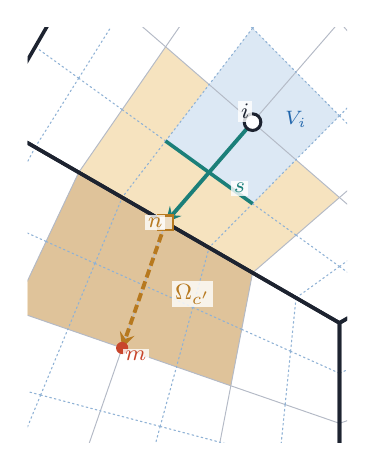
\begin{tikzpicture}[scale=3.0]
\clip (-1.320,-0.506) rectangle (0.032,1.250);
\fill[gradfill] (-0.368,0.212) -- (-0.736,0.425) -- (-0.368,0.850) -- (-0.000,0.531) -- cycle;
\fill[gradfill] (-0.736,0.425) -- (-1.104,0.637) -- (-0.736,1.169) -- (-0.368,0.850) -- cycle;
\fill[gradfill] (-0.368,0.212) -- (-0.460,-0.266) -- (-0.920,-0.106) -- (-0.736,0.425) -- cycle;
\fill[gradfill] (-0.736,0.425) -- (-0.920,-0.106) -- (-1.380,0.053) -- (-1.104,0.637) -- cycle;
\fill[gradstrong] (-0.368,0.212) -- (-0.460,-0.266) -- (-0.920,-0.106) -- (-0.736,0.425) -- cycle;
\fill[gradstrong] (-0.736,0.425) -- (-0.920,-0.106) -- (-1.380,0.053) -- (-1.104,0.637) -- cycle;
\fill[cvfill] (-0.368,0.850) -- (-0.184,0.691) -- (-0.368,0.505) -- (-0.552,0.637) -- cycle;
\fill[cvfill] (-0.368,0.850) -- (-0.552,0.637) -- (-0.736,0.770) -- (-0.552,1.009) -- cycle;
\fill[cvfill] (-0.368,0.850) -- (-0.184,1.062) -- (-0.000,0.877) -- (-0.184,0.691) -- cycle;
\fill[cvfill] (-0.368,0.850) -- (-0.552,1.009) -- (-0.368,1.248) -- (-0.184,1.062) -- cycle;
\draw[micro] (0.000,0.000) -- (-0.368,0.212);
\draw[micro] (-0.368,0.212) -- (-0.000,0.531);
\draw[micro] (-0.000,0.531) -- (0.368,0.212);
\draw[micro] (0.368,0.212) -- (0.000,0.000);
\draw[micro] (-0.368,0.212) -- (-0.736,0.425);
\draw[micro] (-0.736,0.425) -- (-0.368,0.850);
\draw[micro] (-0.368,0.850) -- (-0.000,0.531);
\draw[micro] (-0.736,0.425) -- (-1.104,0.637);
\draw[micro] (-1.104,0.637) -- (-0.736,1.169);
\draw[micro] (-0.736,1.169) -- (-0.368,0.850);
\draw[micro] (-1.104,0.637) -- (-1.472,0.850);
\draw[micro] (-1.472,0.850) -- (-1.104,1.487);
\draw[micro] (-1.104,1.487) -- (-0.736,1.169);
\draw[micro] (-0.000,0.531) -- (0.368,0.850);
\draw[micro] (0.368,0.850) -- (0.736,0.425);
\draw[micro] (0.736,0.425) -- (0.368,0.212);
\draw[micro] (-0.368,0.850) -- (-0.000,1.275);
\draw[micro] (-0.000,1.275) -- (0.368,0.850);
\draw[micro] (-0.736,1.169) -- (-0.368,1.700);
\draw[micro] (-0.368,1.700) -- (-0.000,1.275);
\draw[micro] (-1.104,1.487) -- (-0.736,2.125);
\draw[micro] (-0.736,2.125) -- (-0.368,1.700);
\draw[micro] (0.368,0.850) -- (0.736,1.169);
\draw[micro] (0.736,1.169) -- (1.104,0.637);
\draw[micro] (1.104,0.637) -- (0.736,0.425);
\draw[micro] (-0.000,1.275) -- (0.368,1.700);
\draw[micro] (0.368,1.700) -- (0.736,1.169);
\draw[micro] (-0.368,1.700) -- (0.000,2.231);
\draw[micro] (0.000,2.231) -- (0.368,1.700);
\draw[micro] (-0.736,2.125) -- (-0.368,2.762);
\draw[micro] (-0.368,2.762) -- (0.000,2.231);
\draw[micro] (0.736,1.169) -- (1.104,1.487);
\draw[micro] (1.104,1.487) -- (1.472,0.850);
\draw[micro] (1.472,0.850) -- (1.104,0.637);
\draw[micro] (0.368,1.700) -- (0.736,2.125);
\draw[micro] (0.736,2.125) -- (1.104,1.487);
\draw[micro] (0.000,2.231) -- (0.368,2.762);
\draw[micro] (0.368,2.762) -- (0.736,2.125);
\draw[micro] (-0.368,2.762) -- (0.000,3.400);
\draw[micro] (0.000,3.400) -- (0.368,2.762);
\draw[micro] (0.000,0.000) -- (-0.000,-0.425);
\draw[micro] (-0.000,-0.425) -- (-0.460,-0.266);
\draw[micro] (-0.460,-0.266) -- (-0.368,0.212);
\draw[micro] (-0.000,-0.425) -- (-0.000,-0.850);
\draw[micro] (-0.000,-0.850) -- (-0.552,-0.744);
\draw[micro] (-0.552,-0.744) -- (-0.460,-0.266);
\draw[micro] (-0.000,-0.850) -- (-0.000,-1.275);
\draw[micro] (-0.000,-1.275) -- (-0.644,-1.222);
\draw[micro] (-0.644,-1.222) -- (-0.552,-0.744);
\draw[micro] (-0.000,-1.275) -- (-0.000,-1.700);
\draw[micro] (-0.000,-1.700) -- (-0.736,-1.700);
\draw[micro] (-0.736,-1.700) -- (-0.644,-1.222);
\draw[micro] (-0.460,-0.266) -- (-0.920,-0.106);
\draw[micro] (-0.920,-0.106) -- (-0.736,0.425);
\draw[micro] (-0.552,-0.744) -- (-1.104,-0.638);
\draw[micro] (-1.104,-0.638) -- (-0.920,-0.106);
\draw[micro] (-0.644,-1.222) -- (-1.288,-1.169);
\draw[micro] (-1.288,-1.169) -- (-1.104,-0.638);
\draw[micro] (-0.736,-1.700) -- (-1.472,-1.700);
\draw[micro] (-1.472,-1.700) -- (-1.288,-1.169);
\draw[micro] (-0.920,-0.106) -- (-1.380,0.053);
\draw[micro] (-1.380,0.053) -- (-1.104,0.637);
\draw[micro] (-1.104,-0.638) -- (-1.656,-0.531);
\draw[micro] (-1.656,-0.531) -- (-1.380,0.053);
\draw[micro] (-1.288,-1.169) -- (-1.932,-1.116);
\draw[micro] (-1.932,-1.116) -- (-1.656,-0.531);
\draw[micro] (-1.472,-1.700) -- (-2.208,-1.700);
\draw[micro] (-2.208,-1.700) -- (-1.932,-1.116);
\draw[micro] (-1.380,0.053) -- (-1.840,0.212);
\draw[micro] (-1.840,0.212) -- (-1.472,0.850);
\draw[micro] (-1.656,-0.531) -- (-2.208,-0.425);
\draw[micro] (-2.208,-0.425) -- (-1.840,0.212);
\draw[micro] (-1.932,-1.116) -- (-2.576,-1.063);
\draw[micro] (-2.576,-1.063) -- (-2.208,-0.425);
\draw[micro] (-2.208,-1.700) -- (-2.944,-1.700);
\draw[micro] (-2.944,-1.700) -- (-2.576,-1.063);
\draw[micro] (0.368,0.212) -- (0.460,-0.266);
\draw[micro] (0.460,-0.266) -- (-0.000,-0.425);
\draw[micro] (0.736,0.425) -- (0.920,-0.106);
\draw[micro] (0.920,-0.106) -- (0.460,-0.266);
\draw[micro] (1.104,0.637) -- (1.380,0.053);
\draw[micro] (1.380,0.053) -- (0.920,-0.106);
\draw[micro] (1.472,0.850) -- (1.840,0.212);
\draw[micro] (1.840,0.212) -- (1.380,0.053);
\draw[micro] (0.460,-0.266) -- (0.552,-0.744);
\draw[micro] (0.552,-0.744) -- (-0.000,-0.850);
\draw[micro] (0.920,-0.106) -- (1.104,-0.638);
\draw[micro] (1.104,-0.638) -- (0.552,-0.744);
\draw[micro] (1.380,0.053) -- (1.656,-0.531);
\draw[micro] (1.656,-0.531) -- (1.104,-0.638);
\draw[micro] (1.840,0.212) -- (2.208,-0.425);
\draw[micro] (2.208,-0.425) -- (1.656,-0.531);
\draw[micro] (0.552,-0.744) -- (0.644,-1.222);
\draw[micro] (0.644,-1.222) -- (-0.000,-1.275);
\draw[micro] (1.104,-0.638) -- (1.288,-1.169);
\draw[micro] (1.288,-1.169) -- (0.644,-1.222);
\draw[micro] (1.656,-0.531) -- (1.932,-1.116);
\draw[micro] (1.932,-1.116) -- (1.288,-1.169);
\draw[micro] (2.208,-0.425) -- (2.576,-1.063);
\draw[micro] (2.576,-1.063) -- (1.932,-1.116);
\draw[micro] (0.644,-1.222) -- (0.736,-1.700);
\draw[micro] (0.736,-1.700) -- (-0.000,-1.700);
\draw[micro] (1.288,-1.169) -- (1.472,-1.700);
\draw[micro] (1.472,-1.700) -- (0.736,-1.700);
\draw[micro] (1.932,-1.116) -- (2.208,-1.700);
\draw[micro] (2.208,-1.700) -- (1.472,-1.700);
\draw[micro] (2.576,-1.063) -- (2.944,-1.700);
\draw[micro] (2.944,-1.700) -- (2.208,-1.700);
\draw[dual] (-0.000,0.239) -- (-0.184,0.106);
\draw[dual] (-0.000,0.239) -- (-0.184,0.372);
\draw[dual] (-0.000,0.239) -- (0.184,0.372);
\draw[dual] (-0.000,0.239) -- (0.184,0.106);
\draw[dual] (-0.368,0.505) -- (-0.552,0.319);
\draw[dual] (-0.368,0.505) -- (-0.552,0.637);
\draw[dual] (-0.368,0.505) -- (-0.184,0.691);
\draw[dual] (-0.368,0.505) -- (-0.184,0.372);
\draw[dual] (-0.736,0.770) -- (-0.920,0.531);
\draw[dual] (-0.736,0.770) -- (-0.920,0.903);
\draw[dual] (-0.736,0.770) -- (-0.552,1.009);
\draw[dual] (-0.736,0.770) -- (-0.552,0.637);
\draw[dual] (-1.104,1.036) -- (-1.288,0.744);
\draw[dual] (-1.104,1.036) -- (-1.288,1.169);
\draw[dual] (-1.104,1.036) -- (-0.920,1.328);
\draw[dual] (-1.104,1.036) -- (-0.920,0.903);
\draw[dual] (0.368,0.505) -- (0.184,0.372);
\draw[dual] (0.368,0.505) -- (0.184,0.691);
\draw[dual] (0.368,0.505) -- (0.552,0.637);
\draw[dual] (0.368,0.505) -- (0.552,0.319);
\draw[dual] (-0.000,0.877) -- (-0.184,0.691);
\draw[dual] (-0.000,0.877) -- (-0.184,1.062);
\draw[dual] (-0.000,0.877) -- (0.184,1.062);
\draw[dual] (-0.000,0.877) -- (0.184,0.691);
\draw[dual] (-0.368,1.248) -- (-0.552,1.009);
\draw[dual] (-0.368,1.248) -- (-0.552,1.434);
\draw[dual] (-0.368,1.248) -- (-0.184,1.487);
\draw[dual] (-0.368,1.248) -- (-0.184,1.062);
\draw[dual] (-0.736,1.620) -- (-0.920,1.328);
\draw[dual] (-0.736,1.620) -- (-0.920,1.806);
\draw[dual] (-0.736,1.620) -- (-0.552,1.912);
\draw[dual] (-0.736,1.620) -- (-0.552,1.434);
\draw[dual] (0.736,0.770) -- (0.552,0.637);
\draw[dual] (0.736,0.770) -- (0.552,1.009);
\draw[dual] (0.736,0.770) -- (0.920,0.903);
\draw[dual] (0.736,0.770) -- (0.920,0.531);
\draw[dual] (0.368,1.248) -- (0.184,1.062);
\draw[dual] (0.368,1.248) -- (0.184,1.487);
\draw[dual] (0.368,1.248) -- (0.552,1.434);
\draw[dual] (0.368,1.248) -- (0.552,1.009);
\draw[dual] (0.000,1.727) -- (-0.184,1.487);
\draw[dual] (0.000,1.727) -- (-0.184,1.966);
\draw[dual] (0.000,1.727) -- (0.184,1.966);
\draw[dual] (0.000,1.727) -- (0.184,1.487);
\draw[dual] (-0.368,2.205) -- (-0.552,1.912);
\draw[dual] (-0.368,2.205) -- (-0.552,2.444);
\draw[dual] (-0.368,2.205) -- (-0.184,2.497);
\draw[dual] (-0.368,2.205) -- (-0.184,1.966);
\draw[dual] (1.104,1.036) -- (0.920,0.903);
\draw[dual] (1.104,1.036) -- (0.920,1.328);
\draw[dual] (1.104,1.036) -- (1.288,1.169);
\draw[dual] (1.104,1.036) -- (1.288,0.744);
\draw[dual] (0.736,1.620) -- (0.552,1.434);
\draw[dual] (0.736,1.620) -- (0.552,1.912);
\draw[dual] (0.736,1.620) -- (0.920,1.806);
\draw[dual] (0.736,1.620) -- (0.920,1.328);
\draw[dual] (0.368,2.205) -- (0.184,1.966);
\draw[dual] (0.368,2.205) -- (0.184,2.497);
\draw[dual] (0.368,2.205) -- (0.552,2.444);
\draw[dual] (0.368,2.205) -- (0.552,1.912);
\draw[dual] (0.000,2.789) -- (-0.184,2.497);
\draw[dual] (0.000,2.789) -- (-0.184,3.081);
\draw[dual] (0.000,2.789) -- (0.184,3.081);
\draw[dual] (0.000,2.789) -- (0.184,2.497);
\draw[dual] (-0.207,-0.120) -- (-0.000,-0.213);
\draw[dual] (-0.207,-0.120) -- (-0.230,-0.345);
\draw[dual] (-0.207,-0.120) -- (-0.414,-0.027);
\draw[dual] (-0.207,-0.120) -- (-0.184,0.106);
\draw[dual] (-0.253,-0.571) -- (-0.000,-0.638);
\draw[dual] (-0.253,-0.571) -- (-0.276,-0.797);
\draw[dual] (-0.253,-0.571) -- (-0.506,-0.505);
\draw[dual] (-0.253,-0.571) -- (-0.230,-0.345);
\draw[dual] (-0.299,-1.023) -- (-0.000,-1.063);
\draw[dual] (-0.299,-1.023) -- (-0.322,-1.248);
\draw[dual] (-0.299,-1.023) -- (-0.598,-0.983);
\draw[dual] (-0.299,-1.023) -- (-0.276,-0.797);
\draw[dual] (-0.345,-1.474) -- (-0.000,-1.488);
\draw[dual] (-0.345,-1.474) -- (-0.368,-1.700);
\draw[dual] (-0.345,-1.474) -- (-0.690,-1.461);
\draw[dual] (-0.345,-1.474) -- (-0.322,-1.248);
\draw[dual] (-0.621,0.066) -- (-0.414,-0.027);
\draw[dual] (-0.621,0.066) -- (-0.690,-0.186);
\draw[dual] (-0.621,0.066) -- (-0.828,0.159);
\draw[dual] (-0.621,0.066) -- (-0.552,0.319);
\draw[dual] (-0.759,-0.438) -- (-0.506,-0.505);
\draw[dual] (-0.759,-0.438) -- (-0.828,-0.691);
\draw[dual] (-0.759,-0.438) -- (-1.012,-0.372);
\draw[dual] (-0.759,-0.438) -- (-0.690,-0.186);
\draw[dual] (-0.897,-0.943) -- (-0.598,-0.983);
\draw[dual] (-0.897,-0.943) -- (-0.966,-1.195);
\draw[dual] (-0.897,-0.943) -- (-1.196,-0.903);
\draw[dual] (-0.897,-0.943) -- (-0.828,-0.691);
\draw[dual] (-1.035,-1.448) -- (-0.690,-1.461);
\draw[dual] (-1.035,-1.448) -- (-1.104,-1.700);
\draw[dual] (-1.035,-1.448) -- (-1.380,-1.434);
\draw[dual] (-1.035,-1.448) -- (-0.966,-1.195);
\draw[dual] (-1.035,0.252) -- (-0.828,0.159);
\draw[dual] (-1.035,0.252) -- (-1.150,-0.027);
\draw[dual] (-1.035,0.252) -- (-1.242,0.345);
\draw[dual] (-1.035,0.252) -- (-0.920,0.531);
\draw[dual] (-1.265,-0.305) -- (-1.012,-0.372);
\draw[dual] (-1.265,-0.305) -- (-1.380,-0.584);
\draw[dual] (-1.265,-0.305) -- (-1.518,-0.239);
\draw[dual] (-1.265,-0.305) -- (-1.150,-0.027);
\draw[dual] (-1.495,-0.863) -- (-1.196,-0.903);
\draw[dual] (-1.495,-0.863) -- (-1.610,-1.142);
\draw[dual] (-1.495,-0.863) -- (-1.794,-0.823);
\draw[dual] (-1.495,-0.863) -- (-1.380,-0.584);
\draw[dual] (-1.725,-1.421) -- (-1.380,-1.434);
\draw[dual] (-1.725,-1.421) -- (-1.840,-1.700);
\draw[dual] (-1.725,-1.421) -- (-2.070,-1.408);
\draw[dual] (-1.725,-1.421) -- (-1.610,-1.142);
\draw[dual] (-1.449,0.438) -- (-1.242,0.345);
\draw[dual] (-1.449,0.438) -- (-1.610,0.133);
\draw[dual] (-1.449,0.438) -- (-1.656,0.531);
\draw[dual] (-1.449,0.438) -- (-1.288,0.744);
\draw[dual] (-1.771,-0.173) -- (-1.518,-0.239);
\draw[dual] (-1.771,-0.173) -- (-1.932,-0.478);
\draw[dual] (-1.771,-0.173) -- (-2.024,-0.106);
\draw[dual] (-1.771,-0.173) -- (-1.610,0.133);
\draw[dual] (-2.093,-0.784) -- (-1.794,-0.823);
\draw[dual] (-2.093,-0.784) -- (-2.254,-1.089);
\draw[dual] (-2.093,-0.784) -- (-2.392,-0.744);
\draw[dual] (-2.093,-0.784) -- (-1.932,-0.478);
\draw[dual] (-2.415,-1.395) -- (-2.070,-1.408);
\draw[dual] (-2.415,-1.395) -- (-2.576,-1.700);
\draw[dual] (-2.415,-1.395) -- (-2.760,-1.381);
\draw[dual] (-2.415,-1.395) -- (-2.254,-1.089);
\draw[dual] (0.207,-0.120) -- (0.184,0.106);
\draw[dual] (0.207,-0.120) -- (0.414,-0.027);
\draw[dual] (0.207,-0.120) -- (0.230,-0.345);
\draw[dual] (0.207,-0.120) -- (-0.000,-0.213);
\draw[dual] (0.621,0.066) -- (0.552,0.319);
\draw[dual] (0.621,0.066) -- (0.828,0.159);
\draw[dual] (0.621,0.066) -- (0.690,-0.186);
\draw[dual] (0.621,0.066) -- (0.414,-0.027);
\draw[dual] (1.035,0.252) -- (0.920,0.531);
\draw[dual] (1.035,0.252) -- (1.242,0.345);
\draw[dual] (1.035,0.252) -- (1.150,-0.027);
\draw[dual] (1.035,0.252) -- (0.828,0.159);
\draw[dual] (1.449,0.438) -- (1.288,0.744);
\draw[dual] (1.449,0.438) -- (1.656,0.531);
\draw[dual] (1.449,0.438) -- (1.610,0.133);
\draw[dual] (1.449,0.438) -- (1.242,0.345);
\draw[dual] (0.253,-0.571) -- (0.230,-0.345);
\draw[dual] (0.253,-0.571) -- (0.506,-0.505);
\draw[dual] (0.253,-0.571) -- (0.276,-0.797);
\draw[dual] (0.253,-0.571) -- (-0.000,-0.638);
\draw[dual] (0.759,-0.438) -- (0.690,-0.186);
\draw[dual] (0.759,-0.438) -- (1.012,-0.372);
\draw[dual] (0.759,-0.438) -- (0.828,-0.691);
\draw[dual] (0.759,-0.438) -- (0.506,-0.505);
\draw[dual] (1.265,-0.305) -- (1.150,-0.027);
\draw[dual] (1.265,-0.305) -- (1.518,-0.239);
\draw[dual] (1.265,-0.305) -- (1.380,-0.584);
\draw[dual] (1.265,-0.305) -- (1.012,-0.372);
\draw[dual] (1.771,-0.173) -- (1.610,0.133);
\draw[dual] (1.771,-0.173) -- (2.024,-0.106);
\draw[dual] (1.771,-0.173) -- (1.932,-0.478);
\draw[dual] (1.771,-0.173) -- (1.518,-0.239);
\draw[dual] (0.299,-1.023) -- (0.276,-0.797);
\draw[dual] (0.299,-1.023) -- (0.598,-0.983);
\draw[dual] (0.299,-1.023) -- (0.322,-1.248);
\draw[dual] (0.299,-1.023) -- (-0.000,-1.063);
\draw[dual] (0.897,-0.943) -- (0.828,-0.691);
\draw[dual] (0.897,-0.943) -- (1.196,-0.903);
\draw[dual] (0.897,-0.943) -- (0.966,-1.195);
\draw[dual] (0.897,-0.943) -- (0.598,-0.983);
\draw[dual] (1.495,-0.863) -- (1.380,-0.584);
\draw[dual] (1.495,-0.863) -- (1.794,-0.823);
\draw[dual] (1.495,-0.863) -- (1.610,-1.142);
\draw[dual] (1.495,-0.863) -- (1.196,-0.903);
\draw[dual] (2.093,-0.784) -- (1.932,-0.478);
\draw[dual] (2.093,-0.784) -- (2.392,-0.744);
\draw[dual] (2.093,-0.784) -- (2.254,-1.089);
\draw[dual] (2.093,-0.784) -- (1.794,-0.823);
\draw[dual] (0.345,-1.474) -- (0.322,-1.248);
\draw[dual] (0.345,-1.474) -- (0.690,-1.461);
\draw[dual] (0.345,-1.474) -- (0.368,-1.700);
\draw[dual] (0.345,-1.474) -- (-0.000,-1.488);
\draw[dual] (1.035,-1.448) -- (0.966,-1.195);
\draw[dual] (1.035,-1.448) -- (1.380,-1.434);
\draw[dual] (1.035,-1.448) -- (1.104,-1.700);
\draw[dual] (1.035,-1.448) -- (0.690,-1.461);
\draw[dual] (1.725,-1.421) -- (1.610,-1.142);
\draw[dual] (1.725,-1.421) -- (2.070,-1.408);
\draw[dual] (1.725,-1.421) -- (1.840,-1.700);
\draw[dual] (1.725,-1.421) -- (1.380,-1.434);
\draw[dual] (2.415,-1.395) -- (2.254,-1.089);
\draw[dual] (2.415,-1.395) -- (2.760,-1.381);
\draw[dual] (2.415,-1.395) -- (2.576,-1.700);
\draw[dual] (2.415,-1.395) -- (2.070,-1.408);
\draw[macro] (0.000,0.000) -- (-1.472,0.850) -- (0.000,3.400) -- (1.472,0.850) -- cycle;
\draw[macro] (0.000,0.000) -- (-0.000,-1.700) -- (-2.944,-1.700) -- (-1.472,0.850) -- cycle;
\draw[macro] (0.000,0.000) -- (1.472,0.850) -- (2.944,-1.700) -- (-0.000,-1.700) -- cycle;
\draw[kface] (-0.368,0.505) -- (-0.552,0.637);
\draw[kface] (-0.736,0.770) -- (-0.552,0.637);
\node[nodelabel, right] at (-0.460,0.571) {$\cf{s}$};
\draw[kpath] (-0.368,0.850) -- (-0.736,0.425);
\draw[gpath] (-0.736,0.425) -- (-0.920,-0.106);
\node[gradnode] at (-0.736,0.425) {};
\node[cross] at (-0.920,-0.106) {};
\node[rownode] at (-0.368,0.850) {};
\node[nodelabel, above left] at (-0.368,0.850) {$i$};
\node[nodelabel, left] at (-0.736,0.425) {$\cg{n}$};
\node[nodelabel, below right] at (-0.920,-0.106) {$\cx{m}$};
\node[nodelabel, above] at (-0.621,0.066) {$\cg{\Omega_{c'}}$};
\node[cvlabel] at (-0.184,0.863) {$V_i$};
\end{tikzpicture}

\caption{The formulas on the mesh, zoomed. (a) A frozen entry, Eq.~\eqref{eq:jac} first group
($\cv{A_{\text{frozen}}}$): in the element $\Omega_c$ (grey, solid edges) the two faces
\keyline{kface} of the control volume $\cv{V_i}$ (blue, dotted edges) separate $i$ \key{rownode}
from its edge neighbours; each face term reads only the four corners \key{reach} of $\Omega_c$. The arrows are $\bm d_s$ from $i$ to $j$ and the face's area vector $\cf{\bm a_s}$. (b) One
path of Eq.~\eqref{eq:path}: face $\cf{s}$ of $\cv{V_i}$ reads the gradient at $\cg{n}$
\key{gradnode} ($\cf{[K]_{in}}$, \keyline{kpath}); $\cg{\bm g_n}$ averages the shaded cells around
$\cg{n}$ on both sides of the macro-element boundary (thick line; $\cg{W_n}$); the element
$\cg{\Omega_{c'}}$ contains $\cg{n}$ and $\cx{m}$ \key{cross} ($\cg{[G]_{nm}}$, \keyline{gpath}). No macro-element
contains both $i$ and $\cx{m}$, so a macro-element matrix cannot hold this entry.}
\label{fig:anatomy}
\end{figure}

\subsection{The reach of each factor}

The Jacobian therefore has two parts. $\cv{A_{\text{frozen}}}$ treats $\cg{g}$ as given. The
remaining part differentiates through $\cg{g}$ and factors as $\cf{K}\,\cg{W^{-1}G}$,
Eq.~\eqref{eq:factors}:
\begin{itemize}[leftmargin=*, itemsep=2pt]
\item $\cg{G}$ maps nodal pressures to area-weighted cell gradients summed at each node;
\item $\cg{W^{-1}}$ divides by the nodal area --- a diagonal, which reaches nothing;
\item $\cf{K}$ maps the gradient at the two ends of each face into the rows the face flux enters:
continuity, and momentum through the upwind weights.
\end{itemize}

\begin{figure}[h]
\centering
\input{figures/locality_frozen.tex}\hfill
\input{figures/locality_grad.tex}\hfill
\input{figures/locality_k.tex}
\caption{Row reach of each factor on the unstructured mesh. (a) $\cv{A_{\text{frozen}}}$: every
face term of the control volume (dotted outline) reads only the element it lies in, so row $i$
\key{rownode} reaches the \nfrozenNear{} nodes \key{reach} of the shaded elements. (b) $\cg{W^{-1}G}$ at a node $\cg{n}$
\key{gradnode} on the edge shared by $E_0$ and \nbr: it averages the \ngradEdgeCells{} shaded
elements from \emph{both} macro-elements and reads their \ngradEdge{} nodes. (c) $\cf{K}$, row $i$: the
faces \keyline{kface} of $i$'s control volume read the gradient at $i$ and at its edge
neighbours, \nkNear{} gradient nodes \key{gradnode} --- one of which is the shared node of
panel (b).}
\label{fig:factors}
\end{figure}

Each sparse factor reaches one ring of nodes. $\cv{A_{\text{frozen}}}$, $\cg{G}$ and $\cf{K}$ are each a sum
of micro-cell contributions, so each is a sum of macro-element matrices. The difficulty is only
in their product.

\section{The product $K W^{-1} G$}

Row $i$ of the product reaches every node $m$ that the gradient at some $\cg{n}$ in $\cf{K}$'s row reads.
The second ring comes from chaining the two one-ring factors through $n$. Figure~\ref{fig:exact}
colours each reached node by whether a macro-element matrix could hold the entry.

\begin{figure}[h]
\centering
\input{figures/locality_exact_int.tex}\hfill
\input{figures/locality_exact_near.tex}\hfill
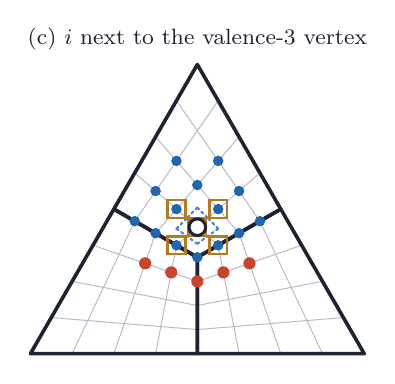
\begin{tikzpicture}[scale=0.72]
\draw[micro] (0.000,0.000) -- (-0.368,0.212);
\draw[micro] (-0.368,0.212) -- (-0.000,0.531);
\draw[micro] (-0.000,0.531) -- (0.368,0.212);
\draw[micro] (0.368,0.212) -- (0.000,0.000);
\draw[micro] (-0.368,0.212) -- (-0.736,0.425);
\draw[micro] (-0.736,0.425) -- (-0.368,0.850);
\draw[micro] (-0.368,0.850) -- (-0.000,0.531);
\draw[micro] (-0.736,0.425) -- (-1.104,0.637);
\draw[micro] (-1.104,0.637) -- (-0.736,1.169);
\draw[micro] (-0.736,1.169) -- (-0.368,0.850);
\draw[micro] (-1.104,0.637) -- (-1.472,0.850);
\draw[micro] (-1.472,0.850) -- (-1.104,1.487);
\draw[micro] (-1.104,1.487) -- (-0.736,1.169);
\draw[micro] (-0.000,0.531) -- (0.368,0.850);
\draw[micro] (0.368,0.850) -- (0.736,0.425);
\draw[micro] (0.736,0.425) -- (0.368,0.212);
\draw[micro] (-0.368,0.850) -- (-0.000,1.275);
\draw[micro] (-0.000,1.275) -- (0.368,0.850);
\draw[micro] (-0.736,1.169) -- (-0.368,1.700);
\draw[micro] (-0.368,1.700) -- (-0.000,1.275);
\draw[micro] (-1.104,1.487) -- (-0.736,2.125);
\draw[micro] (-0.736,2.125) -- (-0.368,1.700);
\draw[micro] (0.368,0.850) -- (0.736,1.169);
\draw[micro] (0.736,1.169) -- (1.104,0.637);
\draw[micro] (1.104,0.637) -- (0.736,0.425);
\draw[micro] (-0.000,1.275) -- (0.368,1.700);
\draw[micro] (0.368,1.700) -- (0.736,1.169);
\draw[micro] (-0.368,1.700) -- (0.000,2.231);
\draw[micro] (0.000,2.231) -- (0.368,1.700);
\draw[micro] (-0.736,2.125) -- (-0.368,2.762);
\draw[micro] (-0.368,2.762) -- (0.000,2.231);
\draw[micro] (0.736,1.169) -- (1.104,1.487);
\draw[micro] (1.104,1.487) -- (1.472,0.850);
\draw[micro] (1.472,0.850) -- (1.104,0.637);
\draw[micro] (0.368,1.700) -- (0.736,2.125);
\draw[micro] (0.736,2.125) -- (1.104,1.487);
\draw[micro] (0.000,2.231) -- (0.368,2.762);
\draw[micro] (0.368,2.762) -- (0.736,2.125);
\draw[micro] (-0.368,2.762) -- (0.000,3.400);
\draw[micro] (0.000,3.400) -- (0.368,2.762);
\draw[micro] (0.000,0.000) -- (-0.000,-0.425);
\draw[micro] (-0.000,-0.425) -- (-0.460,-0.266);
\draw[micro] (-0.460,-0.266) -- (-0.368,0.212);
\draw[micro] (-0.000,-0.425) -- (-0.000,-0.850);
\draw[micro] (-0.000,-0.850) -- (-0.552,-0.744);
\draw[micro] (-0.552,-0.744) -- (-0.460,-0.266);
\draw[micro] (-0.000,-0.850) -- (-0.000,-1.275);
\draw[micro] (-0.000,-1.275) -- (-0.644,-1.222);
\draw[micro] (-0.644,-1.222) -- (-0.552,-0.744);
\draw[micro] (-0.000,-1.275) -- (-0.000,-1.700);
\draw[micro] (-0.000,-1.700) -- (-0.736,-1.700);
\draw[micro] (-0.736,-1.700) -- (-0.644,-1.222);
\draw[micro] (-0.460,-0.266) -- (-0.920,-0.106);
\draw[micro] (-0.920,-0.106) -- (-0.736,0.425);
\draw[micro] (-0.552,-0.744) -- (-1.104,-0.638);
\draw[micro] (-1.104,-0.638) -- (-0.920,-0.106);
\draw[micro] (-0.644,-1.222) -- (-1.288,-1.169);
\draw[micro] (-1.288,-1.169) -- (-1.104,-0.638);
\draw[micro] (-0.736,-1.700) -- (-1.472,-1.700);
\draw[micro] (-1.472,-1.700) -- (-1.288,-1.169);
\draw[micro] (-0.920,-0.106) -- (-1.380,0.053);
\draw[micro] (-1.380,0.053) -- (-1.104,0.637);
\draw[micro] (-1.104,-0.638) -- (-1.656,-0.531);
\draw[micro] (-1.656,-0.531) -- (-1.380,0.053);
\draw[micro] (-1.288,-1.169) -- (-1.932,-1.116);
\draw[micro] (-1.932,-1.116) -- (-1.656,-0.531);
\draw[micro] (-1.472,-1.700) -- (-2.208,-1.700);
\draw[micro] (-2.208,-1.700) -- (-1.932,-1.116);
\draw[micro] (-1.380,0.053) -- (-1.840,0.212);
\draw[micro] (-1.840,0.212) -- (-1.472,0.850);
\draw[micro] (-1.656,-0.531) -- (-2.208,-0.425);
\draw[micro] (-2.208,-0.425) -- (-1.840,0.212);
\draw[micro] (-1.932,-1.116) -- (-2.576,-1.063);
\draw[micro] (-2.576,-1.063) -- (-2.208,-0.425);
\draw[micro] (-2.208,-1.700) -- (-2.944,-1.700);
\draw[micro] (-2.944,-1.700) -- (-2.576,-1.063);
\draw[micro] (0.368,0.212) -- (0.460,-0.266);
\draw[micro] (0.460,-0.266) -- (-0.000,-0.425);
\draw[micro] (0.736,0.425) -- (0.920,-0.106);
\draw[micro] (0.920,-0.106) -- (0.460,-0.266);
\draw[micro] (1.104,0.637) -- (1.380,0.053);
\draw[micro] (1.380,0.053) -- (0.920,-0.106);
\draw[micro] (1.472,0.850) -- (1.840,0.212);
\draw[micro] (1.840,0.212) -- (1.380,0.053);
\draw[micro] (0.460,-0.266) -- (0.552,-0.744);
\draw[micro] (0.552,-0.744) -- (-0.000,-0.850);
\draw[micro] (0.920,-0.106) -- (1.104,-0.638);
\draw[micro] (1.104,-0.638) -- (0.552,-0.744);
\draw[micro] (1.380,0.053) -- (1.656,-0.531);
\draw[micro] (1.656,-0.531) -- (1.104,-0.638);
\draw[micro] (1.840,0.212) -- (2.208,-0.425);
\draw[micro] (2.208,-0.425) -- (1.656,-0.531);
\draw[micro] (0.552,-0.744) -- (0.644,-1.222);
\draw[micro] (0.644,-1.222) -- (-0.000,-1.275);
\draw[micro] (1.104,-0.638) -- (1.288,-1.169);
\draw[micro] (1.288,-1.169) -- (0.644,-1.222);
\draw[micro] (1.656,-0.531) -- (1.932,-1.116);
\draw[micro] (1.932,-1.116) -- (1.288,-1.169);
\draw[micro] (2.208,-0.425) -- (2.576,-1.063);
\draw[micro] (2.576,-1.063) -- (1.932,-1.116);
\draw[micro] (0.644,-1.222) -- (0.736,-1.700);
\draw[micro] (0.736,-1.700) -- (-0.000,-1.700);
\draw[micro] (1.288,-1.169) -- (1.472,-1.700);
\draw[micro] (1.472,-1.700) -- (0.736,-1.700);
\draw[micro] (1.932,-1.116) -- (2.208,-1.700);
\draw[micro] (2.208,-1.700) -- (1.472,-1.700);
\draw[micro] (2.576,-1.063) -- (2.944,-1.700);
\draw[micro] (2.944,-1.700) -- (2.208,-1.700);
\draw[macro] (0.000,0.000) -- (-1.472,0.850) -- (0.000,3.400) -- (1.472,0.850) -- cycle;
\draw[macro] (0.000,0.000) -- (-0.000,-1.700) -- (-2.944,-1.700) -- (-1.472,0.850) -- cycle;
\draw[macro] (0.000,0.000) -- (1.472,0.850) -- (2.944,-1.700) -- (-0.000,-1.700) -- cycle;
\draw[cvline] (-0.000,0.239) -- (0.184,0.372);
\draw[cvline] (-0.000,0.239) -- (-0.184,0.372);
\draw[cvline] (-0.368,0.505) -- (-0.184,0.372);
\draw[cvline] (-0.368,0.505) -- (-0.184,0.691);
\draw[cvline] (0.368,0.505) -- (0.184,0.691);
\draw[cvline] (0.368,0.505) -- (0.184,0.372);
\draw[cvline] (-0.000,0.877) -- (-0.184,0.691);
\draw[cvline] (-0.000,0.877) -- (0.184,0.691);
\node[reach] at (0.000,0.000) {};
\node[reach] at (-0.368,0.212) {};
\node[reach] at (-0.736,0.425) {};
\node[reach] at (-1.104,0.637) {};
\node[reach] at (0.368,0.212) {};
\node[reach] at (-0.000,0.531) {};
\node[reach] at (-0.368,0.850) {};
\node[reach] at (-0.736,1.169) {};
\node[reach] at (0.736,0.425) {};
\node[reach] at (0.368,0.850) {};
\node[reach] at (-0.000,1.275) {};
\node[reach] at (-0.368,1.700) {};
\node[reach] at (1.104,0.637) {};
\node[reach] at (0.736,1.169) {};
\node[reach] at (0.368,1.700) {};
\node[cross] at (-0.000,-0.425) {};
\node[cross] at (-0.460,-0.266) {};
\node[cross] at (-0.920,-0.106) {};
\node[cross] at (0.460,-0.266) {};
\node[cross] at (0.920,-0.106) {};
\node[gradring] at (-0.368,0.212) {};
\node[gradring] at (0.368,0.212) {};
\node[gradring] at (-0.000,0.531) {};
\node[gradring] at (-0.368,0.850) {};
\node[gradring] at (0.368,0.850) {};
\node[rownode] at (-0.000,0.531) {};
\node[panel, anchor=south] at (0.000,3.650) {(c) $i$ next to the valence-3 vertex};
\end{tikzpicture}

\caption{Row $i$ \key{rownode} of $\cf{K}\,\cg{W^{-1} G}$, through the gradient nodes
\key{gradring} of $\cf{K}$'s row. \key{reach} some macro-element contains both $i$ and $m$;
\key{cross} none does. (a) $i$ inside $E_0$: \nexactInt{} nodes, \ncrossInt{} red. (b) One step
from the edge shared with \nbr: \nexactNear{} nodes, \ncrossNear{} red --- the gradient at the
shared node reads the cells of \nbr. (c) One step from the valence-3 vertex: \nexactCorner{} nodes,
\ncrossCorner{} red, reaching into both neighbours. $\cv{A_{\text{frozen}}}$ reaches \nfrozenInt{},
\nfrozenNear{} and \nfrozenCorner{} nodes at the same three rows, none red.}
\label{fig:exact}
\end{figure}

This is exactly what the element-locality gate in the driver measures: a direction placed on the
interior of one macro-element produces a response in its neighbours only through this term.
The matrix-free Jacobian includes the red entries, because its gradient pass and its face pass
both run over every macro-element and sum at shared nodes. The element-wise assembly omits the
whole term --- the blue entries as well as the red ones --- and could only ever add the blue.

\subsection{How the exact operator is applied}

The product $\cf{K}\,\cg{W^{-1}G}$ is never formed. The matrix-free Jacobian applies its two factors
in two passes, exactly as the path sum~\eqref{eq:path} suggests: first $\cg{W^{-1}G}$ acts on the
pressure of the direction, producing a nodal gradient $\cg{\bm g^q}$ at every node
(Algorithm~\ref{alg:grad}); then the face loop applies $\cf{K}$ by reading that gradient at the two
ends of each face (Algorithm~\ref{alg:apply}). Both passes run macro-element by macro-element and
sum shared nodes with the deterministic two-pass scatter, so the gradient at a node on a
macro-element boundary contains every element around it --- which is how the red entries enter
the action. Algorithm~\ref{alg:apply} follows \code{sscvfem\_apply},
\code{sscvfem\_apply\_macro\_local\_hoisted} and \code{sscvfem\_action\_hoisted}; the
three-dimensional code has the same structure with twelve faces per element.

\begin{algorithm}[H]
\caption{Nodal gradient $\cg{\bm g} = \cg{W^{-1}G}\,q$ \quad (\code{sscvfem\_nodal\_grad\_strided}),
Eq.~\eqref{eq:grad}}\label{alg:grad}
\begin{algorithmic}[1]
\Function{NodalGradient}{$q$}
  \State $\cg{\bm g_n} \gets \bm 0$ for every node $n$
  \ForAll{macro-elements $E$ \textbf{in parallel}}
    \State gather $q$ at the nodes of $E$
    \ForAll{elements $\Omega_c \subset E$}
      \State $\cg{\bm\gamma_c} \gets |\Omega_c|\,\nabla q\big|_c = |\Omega_c|\sum_{a\in c} q_a\,\nabla N_a\big|_c$
        \Comment{only the sign of the determinant survives}
      \ForAll{corners $a$ of $\Omega_c$}
        \State $\cg{\bm g_a} \gets \cg{\bm g_a} + \cg{\bm\gamma_c}$ \Comment{local to $E$}
      \EndFor
    \EndFor
    \State scatter: write nodes owned by $E$ alone; stage nodes shared with other macro-elements
  \EndFor
  \State reduce every shared node: sum its staged contributions in a fixed order
  \ForAll{nodes $n$}
    \State $\cg{\bm g_n} \gets \cg{W_n^{-1}}\,\cg{\bm g_n}$, \quad
      $\cg{W_n} = \sum_{c\ni n}|\Omega_c|$ \Comment{cached once per mesh}
  \EndFor
  \State \Return $\cg{\bm g}$
\EndFunction
\end{algorithmic}
\end{algorithm}

\begin{algorithm}[H]
\caption{Exact Jacobian action $y = J_{\text{exact}}(u,p)\,(v,q)$ \quad (\code{sscvfem\_apply}),
Eq.~\eqref{eq:jac}}\label{alg:apply}
\begin{algorithmic}[1]
\Require state $(u,p)$ with its nodal gradient $\bm g^p$ (from the last update); direction $(v,q)$
\State $\cg{\bm g^q} \gets$ \Call{NodalGradient}{$q$}
  \Comment{the one extra pass; omitted, this is $\cv{A_{\text{frozen}}}$}
\State $y \gets 0$
\ForAll{macro-elements $E$ \textbf{in parallel}}
  \State gather $\bm x, u, p, \bm g^p, v, q, \cg{\bm g^q}$ at the nodes of $E$
  \ForAll{elements $\Omega_c \subset E$}
    \State \cv{viscous: traction of $\nabla v|_c$ on each face of $\Omega_c$, into the momentum rows of its two nodes}
    \ForAll{faces $\cf{s}$ of $\Omega_c$, separating nodes $i$ and $j$}
      \State $\bar{\bm u} \gets \tfrac12(u_i+u_j)$, \quad $\bar{\bm v} \gets \tfrac12(v_i+v_j)$, \quad
        $c_s \gets$ Rhie--Chow coefficient at $|\bar{\bm u}|$
      \State $\mathrm{corr} \gets (p_j-p_i) - \tfrac12(\bm g^p_i+\bm g^p_j)\cdot\bm d_s$
        \Comment{state, Eq.~\eqref{eq:mdot}}
      \State $\cf{\dot m_s} \gets \rho\,\bar{\bm u}\cdot\cf{\bm a_s} - c_s\,\mathrm{corr}$; \quad
        upwind split $m^\pm$, $\delta^\pm$ from its sign
      \State $\cf{\delta\dot m_s} \gets \cv{\rho\,\bar{\bm v}\cdot\bm a_s + c_s(q_i-q_j) + c_s'\,\mathrm{corr}\,(\bar{\bm u}\cdot\bar{\bm v})}$
      \State \hspace{3.1em} $+\;\cf{\tfrac12\,c_s\,\bm d_s}\cdot(\cg{\bm g^q_i+\bm g^q_j})$
        \Comment{the $\cf{K}\,\cg{W^{-1}G}$ term, Eq.~\eqref{eq:path}}
      \State $\bm f \gets \delta^+\cf{\delta\dot m_s}\,u_i + m^+ v_i + \delta^-\cf{\delta\dot m_s}\,u_j + m^- v_j
        + \tfrac12(q_i+q_j)\,\cf{\bm a_s}$
      \State $y^u_i \mathrel{+}= \bm f$, \; $y^u_j \mathrel{-}= \bm f$, \;
        $y^p_i \mathrel{+}= \cf{\delta\dot m_s}$, \; $y^p_j \mathrel{-}= \cf{\delta\dot m_s}$
    \EndFor
    \State add the linearised flux of any domain-boundary faces of $\Omega_c$
  \EndFor
  \State scatter the local rows of $E$ (owned nodes written, shared nodes staged)
\EndFor
\State reduce every shared node in a fixed order
\State $y^u \mathrel{+}= \rho\,|V|\,a_0/\Delta t\; v$ \Comment{transient term, only when $\Delta t>0$}
\State \Return $y$
\end{algorithmic}
\end{algorithm}

Two properties of this structure matter for everything above. First, the only non-local step is
the one marked $\cg{W^{-1}G}$: remove line~1 of Algorithm~\ref{alg:apply} and every term reads the
corners of a single element, which is $\cv{A_{\text{frozen}}}$ and what the element-wise assembly
builds (\code{SFEM\_RC\_EXACT\_JAC=0} does exactly this). Second, the cost of exactness is one
gradient pass per application, not a wider matrix: the red entries of Figure~\ref{fig:exact} are
applied without ever being stored.

\subsection{How the frozen Jacobian is applied and assembled}

The frozen Jacobian $\cv{A_{\text{frozen}}}$ exists in two forms, and they are the same operator.

\paragraph{Applied, matrix-free.} Algorithm~\ref{alg:apply} with line~1 removed and
$\cg{\bm g^q}=\bm 0$. The state's gradient $\bm g^p$ is still read --- it sets the mass flux and
the upwind direction --- but only as data: nothing differentiates through it. This is the action
\code{SFEM\_RC\_EXACT\_JAC=0} selects.

\paragraph{Assembled, element by element.} Because every remaining term reads the corners of one
element, $\cv{A_{\text{frozen}}}$ is a sum of element matrices, and that is how the Vanka patches
and every Galerkin coarse level are built (\code{galerkin\_assemble},
\code{galerkin\_accumulate}). Algorithm~\ref{alg:elem} writes the element matrix: its entries are
the derivatives of the frozen face terms of Algorithm~\ref{alg:apply} with respect to the
direction, with $\bm w = \delta^+ u_i + \delta^- u_j$ the upwind-weighted velocity of face
$\cf{s}$. Algorithm~\ref{alg:asm} assembles them, contracting each with the prolongation restricted
to the element: at ratio $q=1$ that restriction is the identity and the result is
$\cv{A_{\text{frozen}}}$ itself, which the Vanka smoother reads; at $q>1$ it is the Galerkin coarse
operator $P^{\mathsf T}\cv{A_{\text{frozen}}}P$. Assembly and action agree: at $q=1$ the assembled
matrix reproduces the matrix-free frozen action to $1.5$--$1.7\times10^{-16}$ on the closed box,
the open outlet, the pressure port, the manufactured solution and the warped nozzle
(\code{SFEM\_GMG\_CHECK=1}, job 4670644).

\begin{algorithm}[H]
\caption{Frozen element matrix $\cv{A_c}$ of element $\Omega_c$, $4\times4$ blocks
$\cv{A_c[a,b]}$ for corners $a,b$ (\code{cvfem\_hex8\_ns\_upwind\_jacobian\_add\_slots})}\label{alg:elem}
\begin{algorithmic}[1]
\Require state $u, p$ and its nodal gradient $\bm g^p$ at the corners of $\Omega_c$ (data only)
\State $\cv{A_c} \gets 0$
\State \cv{viscous: for each face of $\Omega_c$, the traction of $\nabla v|_c$ gives the velocity--velocity blocks of its two nodes}
\ForAll{faces $\cf{s}$ of $\Omega_c$, separating corners $i$ and $j$}
  \State $\bar{\bm u},\ c_s,\ \mathrm{corr},\ \cf{\dot m_s},\ m^\pm,\ \delta^\pm$ \; as in Algorithm~\ref{alg:apply}
    \Comment{$\bm g^p$ read, not differentiated}
  \State $\bm b \gets \tfrac12\rho\,\cf{\bm a_s} + \tfrac12\,c_s'\,\mathrm{corr}\,\bar{\bm u}$
    \Comment{$\partial\cf{\delta\dot m_s}/\partial v_i = \partial\cf{\delta\dot m_s}/\partial v_j$}
  \State $\bm w \gets \delta^+ u_i + \delta^- u_j$
  \For{$(k,\sigma) \in \{(i,+1),\ (j,-1)\}$}
    \Comment{row $i$ gains the face flux, row $j$ loses it}
    \State $\cv{A_c[k, i]^{uu}} \mathrel{+}= \sigma\,(\bm w\,\bm b^{\mathsf T} + m^+ I)$, \quad
           $\cv{A_c[k, j]^{uu}} \mathrel{+}= \sigma\,(\bm w\,\bm b^{\mathsf T} + m^- I)$
    \State $\cv{A_c[k, i]^{up}} \mathrel{+}= \sigma\,(c_s\,\bm w + \tfrac12\cf{\bm a_s})$, \quad
           $\cv{A_c[k, j]^{up}} \mathrel{+}= \sigma\,(-c_s\,\bm w + \tfrac12\cf{\bm a_s})$
    \State $\cv{A_c[k, i]^{pu}} \mathrel{+}= \sigma\,\bm b^{\mathsf T}$, \quad
           $\cv{A_c[k, j]^{pu}} \mathrel{+}= \sigma\,\bm b^{\mathsf T}$
    \State $\cv{A_c[k, i]^{pp}} \mathrel{+}= \sigma\,c_s$, \quad
           $\cv{A_c[k, j]^{pp}} \mathrel{+}= -\sigma\,c_s$
  \EndFor
\EndFor
\State \Return $\cv{A_c}$ \Comment{no $\cf{K}\,\cg{W^{-1}G}$: every column is a corner of $\Omega_c$}
\end{algorithmic}
\end{algorithm}

\begin{algorithm}[H]
\caption{Assembly into BSR: $\cv{A_{\text{frozen}}}$ at ratio $q=1$, and
$P^{\mathsf T}\cv{A_{\text{frozen}}}P$ at $q>1$ \quad (\code{galerkin\_assemble})}\label{alg:asm}
\begin{algorithmic}[1]
\Require ratio $q$; fine constraint mask; the level's BSR pattern, derived from the lattice once
  and cached across Newton steps
\State values $\gets 0$
\ForAll{chunks of macro-elements, in a fixed order}
  \ForAll{macro-elements $E$ in the chunk \textbf{in parallel}}
    \State gather $\bm x, u, p, \bm g^p$ at the nodes of $E$; hoist the element geometry
    \ForAll{elements $\Omega_c \subset E$}
      \State $\cv{A_c} \gets$ Algorithm~\ref{alg:elem}
      \State add the transient term $\rho\,a_0/\Delta t\cdot|\Omega_c|/8$ to each corner's velocity diagonal
      \State add the Jacobian of any domain-boundary faces of $\Omega_c$
      \State zero the columns of constrained fine unknowns
        \Comment{gives $P^{\mathsf T}(\cv{A}Z)P$}
      \State $Q \gets$ prolongation restricted to $\Omega_c$ \Comment{$8\times8$ weights; identity at $q=1$}
      \State $C_E[a, b] \mathrel{+}= \sum_{i,j} Q_{ia}\,\cv{A_c[i,j]}\,Q_{jb}$
        \Comment{coarse patch corners $a,b$; 27 fixed slots}
    \EndFor
  \EndFor
  \State accumulate every slot of the chunk into its BSR block, through the cached inverse index
\EndFor
\State \Return BSR(pattern, values) \Comment{caller patches coarse identity rows}
\end{algorithmic}
\end{algorithm}

Set beside Algorithm~\ref{alg:apply}, the difference is exactly one line and one kind of column. The
exact action reads $\cg{\bm g^q}$, a quantity computed from every element around a node; the frozen
Jacobian never does, so each of its columns is a corner of the element being assembled, and the
fixed 27-slot storage of Algorithm~\ref{alg:asm} is enough to hold it.

\section{One coarse level}

The coarse levels are Galerkin operators $P^{\mathsf T} J P$, with $P$ the bilinear interpolation
from a lattice of half the resolution in each macro-element. Figure~\ref{fig:coarse} shows one
coarse row.

\begin{figure}[h]
\centering
\input{figures/locality_coarse_int_frozen.tex}\hspace{2em}
\input{figures/locality_coarse_int_exact.tex}
\caption{Row of the coarse node $I$ \key{rownode} at the centre of $E_0$; small grey dots
\key{support} are the fine nodes where its basis is non-zero, thick grey lines the coarse
lattice. (a) The coarse operator built today, $P^{\mathsf T}A_{\text{frozen}}P$:
\ncoarseFrozenInt{} coarse nodes, \ncoarseCrossFrozenInt{} red. (b) The Galerkin operator of the
exact Jacobian: \ncoarseExactInt{} coarse nodes, \ncoarseCrossExactInt{} red. A coarse node on
the shared edge reaches \ncoarseFrozenEdge{} and \ncoarseExactEdge{} coarse nodes respectively.}
\label{fig:coarse}
\end{figure}

\section{The same operators on a standard quad4 mesh}

On a standard unstructured quad4 mesh every micro-cell is its own element, so an element matrix
holds only the four nodes of one cell. Figure~\ref{fig:quad4} draws the same rows on the same
geometry with that element structure.

\begin{figure}[h]
\centering
\input{figures/locality_quad4_frozen.tex}\hfill
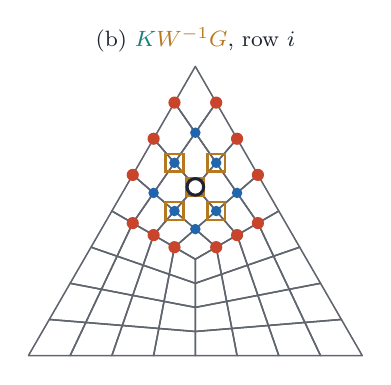
\begin{tikzpicture}[scale=0.72]
\draw[micro] (0.000,0.000) -- (-0.368,0.212);
\draw[micro] (-0.368,0.212) -- (-0.000,0.531);
\draw[micro] (-0.000,0.531) -- (0.368,0.212);
\draw[micro] (0.368,0.212) -- (0.000,0.000);
\draw[micro] (-0.368,0.212) -- (-0.736,0.425);
\draw[micro] (-0.736,0.425) -- (-0.368,0.850);
\draw[micro] (-0.368,0.850) -- (-0.000,0.531);
\draw[micro] (-0.736,0.425) -- (-1.104,0.637);
\draw[micro] (-1.104,0.637) -- (-0.736,1.169);
\draw[micro] (-0.736,1.169) -- (-0.368,0.850);
\draw[micro] (-1.104,0.637) -- (-1.472,0.850);
\draw[micro] (-1.472,0.850) -- (-1.104,1.487);
\draw[micro] (-1.104,1.487) -- (-0.736,1.169);
\draw[micro] (-0.000,0.531) -- (0.368,0.850);
\draw[micro] (0.368,0.850) -- (0.736,0.425);
\draw[micro] (0.736,0.425) -- (0.368,0.212);
\draw[micro] (-0.368,0.850) -- (-0.000,1.275);
\draw[micro] (-0.000,1.275) -- (0.368,0.850);
\draw[micro] (-0.736,1.169) -- (-0.368,1.700);
\draw[micro] (-0.368,1.700) -- (-0.000,1.275);
\draw[micro] (-1.104,1.487) -- (-0.736,2.125);
\draw[micro] (-0.736,2.125) -- (-0.368,1.700);
\draw[micro] (0.368,0.850) -- (0.736,1.169);
\draw[micro] (0.736,1.169) -- (1.104,0.637);
\draw[micro] (1.104,0.637) -- (0.736,0.425);
\draw[micro] (-0.000,1.275) -- (0.368,1.700);
\draw[micro] (0.368,1.700) -- (0.736,1.169);
\draw[micro] (-0.368,1.700) -- (0.000,2.231);
\draw[micro] (0.000,2.231) -- (0.368,1.700);
\draw[micro] (-0.736,2.125) -- (-0.368,2.762);
\draw[micro] (-0.368,2.762) -- (0.000,2.231);
\draw[micro] (0.736,1.169) -- (1.104,1.487);
\draw[micro] (1.104,1.487) -- (1.472,0.850);
\draw[micro] (1.472,0.850) -- (1.104,0.637);
\draw[micro] (0.368,1.700) -- (0.736,2.125);
\draw[micro] (0.736,2.125) -- (1.104,1.487);
\draw[micro] (0.000,2.231) -- (0.368,2.762);
\draw[micro] (0.368,2.762) -- (0.736,2.125);
\draw[micro] (-0.368,2.762) -- (0.000,3.400);
\draw[micro] (0.000,3.400) -- (0.368,2.762);
\draw[micro] (0.000,0.000) -- (-0.000,-0.425);
\draw[micro] (-0.000,-0.425) -- (-0.460,-0.266);
\draw[micro] (-0.460,-0.266) -- (-0.368,0.212);
\draw[micro] (-0.000,-0.425) -- (-0.000,-0.850);
\draw[micro] (-0.000,-0.850) -- (-0.552,-0.744);
\draw[micro] (-0.552,-0.744) -- (-0.460,-0.266);
\draw[micro] (-0.000,-0.850) -- (-0.000,-1.275);
\draw[micro] (-0.000,-1.275) -- (-0.644,-1.222);
\draw[micro] (-0.644,-1.222) -- (-0.552,-0.744);
\draw[micro] (-0.000,-1.275) -- (-0.000,-1.700);
\draw[micro] (-0.000,-1.700) -- (-0.736,-1.700);
\draw[micro] (-0.736,-1.700) -- (-0.644,-1.222);
\draw[micro] (-0.460,-0.266) -- (-0.920,-0.106);
\draw[micro] (-0.920,-0.106) -- (-0.736,0.425);
\draw[micro] (-0.552,-0.744) -- (-1.104,-0.638);
\draw[micro] (-1.104,-0.638) -- (-0.920,-0.106);
\draw[micro] (-0.644,-1.222) -- (-1.288,-1.169);
\draw[micro] (-1.288,-1.169) -- (-1.104,-0.638);
\draw[micro] (-0.736,-1.700) -- (-1.472,-1.700);
\draw[micro] (-1.472,-1.700) -- (-1.288,-1.169);
\draw[micro] (-0.920,-0.106) -- (-1.380,0.053);
\draw[micro] (-1.380,0.053) -- (-1.104,0.637);
\draw[micro] (-1.104,-0.638) -- (-1.656,-0.531);
\draw[micro] (-1.656,-0.531) -- (-1.380,0.053);
\draw[micro] (-1.288,-1.169) -- (-1.932,-1.116);
\draw[micro] (-1.932,-1.116) -- (-1.656,-0.531);
\draw[micro] (-1.472,-1.700) -- (-2.208,-1.700);
\draw[micro] (-2.208,-1.700) -- (-1.932,-1.116);
\draw[micro] (-1.380,0.053) -- (-1.840,0.212);
\draw[micro] (-1.840,0.212) -- (-1.472,0.850);
\draw[micro] (-1.656,-0.531) -- (-2.208,-0.425);
\draw[micro] (-2.208,-0.425) -- (-1.840,0.212);
\draw[micro] (-1.932,-1.116) -- (-2.576,-1.063);
\draw[micro] (-2.576,-1.063) -- (-2.208,-0.425);
\draw[micro] (-2.208,-1.700) -- (-2.944,-1.700);
\draw[micro] (-2.944,-1.700) -- (-2.576,-1.063);
\draw[micro] (0.368,0.212) -- (0.460,-0.266);
\draw[micro] (0.460,-0.266) -- (-0.000,-0.425);
\draw[micro] (0.736,0.425) -- (0.920,-0.106);
\draw[micro] (0.920,-0.106) -- (0.460,-0.266);
\draw[micro] (1.104,0.637) -- (1.380,0.053);
\draw[micro] (1.380,0.053) -- (0.920,-0.106);
\draw[micro] (1.472,0.850) -- (1.840,0.212);
\draw[micro] (1.840,0.212) -- (1.380,0.053);
\draw[micro] (0.460,-0.266) -- (0.552,-0.744);
\draw[micro] (0.552,-0.744) -- (-0.000,-0.850);
\draw[micro] (0.920,-0.106) -- (1.104,-0.638);
\draw[micro] (1.104,-0.638) -- (0.552,-0.744);
\draw[micro] (1.380,0.053) -- (1.656,-0.531);
\draw[micro] (1.656,-0.531) -- (1.104,-0.638);
\draw[micro] (1.840,0.212) -- (2.208,-0.425);
\draw[micro] (2.208,-0.425) -- (1.656,-0.531);
\draw[micro] (0.552,-0.744) -- (0.644,-1.222);
\draw[micro] (0.644,-1.222) -- (-0.000,-1.275);
\draw[micro] (1.104,-0.638) -- (1.288,-1.169);
\draw[micro] (1.288,-1.169) -- (0.644,-1.222);
\draw[micro] (1.656,-0.531) -- (1.932,-1.116);
\draw[micro] (1.932,-1.116) -- (1.288,-1.169);
\draw[micro] (2.208,-0.425) -- (2.576,-1.063);
\draw[micro] (2.576,-1.063) -- (1.932,-1.116);
\draw[micro] (0.644,-1.222) -- (0.736,-1.700);
\draw[micro] (0.736,-1.700) -- (-0.000,-1.700);
\draw[micro] (1.288,-1.169) -- (1.472,-1.700);
\draw[micro] (1.472,-1.700) -- (0.736,-1.700);
\draw[micro] (1.932,-1.116) -- (2.208,-1.700);
\draw[micro] (2.208,-1.700) -- (1.472,-1.700);
\draw[micro] (2.576,-1.063) -- (2.944,-1.700);
\draw[micro] (2.944,-1.700) -- (2.208,-1.700);
\draw[element] (0.000,0.000) -- (-0.368,0.212) -- (-0.000,0.531) -- (0.368,0.212) -- cycle;
\draw[element] (-0.368,0.212) -- (-0.736,0.425) -- (-0.368,0.850) -- (-0.000,0.531) -- cycle;
\draw[element] (-0.736,0.425) -- (-1.104,0.637) -- (-0.736,1.169) -- (-0.368,0.850) -- cycle;
\draw[element] (-1.104,0.637) -- (-1.472,0.850) -- (-1.104,1.487) -- (-0.736,1.169) -- cycle;
\draw[element] (0.368,0.212) -- (-0.000,0.531) -- (0.368,0.850) -- (0.736,0.425) -- cycle;
\draw[element] (-0.000,0.531) -- (-0.368,0.850) -- (-0.000,1.275) -- (0.368,0.850) -- cycle;
\draw[element] (-0.368,0.850) -- (-0.736,1.169) -- (-0.368,1.700) -- (-0.000,1.275) -- cycle;
\draw[element] (-0.736,1.169) -- (-1.104,1.487) -- (-0.736,2.125) -- (-0.368,1.700) -- cycle;
\draw[element] (0.736,0.425) -- (0.368,0.850) -- (0.736,1.169) -- (1.104,0.637) -- cycle;
\draw[element] (0.368,0.850) -- (-0.000,1.275) -- (0.368,1.700) -- (0.736,1.169) -- cycle;
\draw[element] (-0.000,1.275) -- (-0.368,1.700) -- (0.000,2.231) -- (0.368,1.700) -- cycle;
\draw[element] (-0.368,1.700) -- (-0.736,2.125) -- (-0.368,2.762) -- (0.000,2.231) -- cycle;
\draw[element] (1.104,0.637) -- (0.736,1.169) -- (1.104,1.487) -- (1.472,0.850) -- cycle;
\draw[element] (0.736,1.169) -- (0.368,1.700) -- (0.736,2.125) -- (1.104,1.487) -- cycle;
\draw[element] (0.368,1.700) -- (0.000,2.231) -- (0.368,2.762) -- (0.736,2.125) -- cycle;
\draw[element] (0.000,2.231) -- (-0.368,2.762) -- (0.000,3.400) -- (0.368,2.762) -- cycle;
\draw[element] (0.000,0.000) -- (-0.000,-0.425) -- (-0.460,-0.266) -- (-0.368,0.212) -- cycle;
\draw[element] (-0.000,-0.425) -- (-0.000,-0.850) -- (-0.552,-0.744) -- (-0.460,-0.266) -- cycle;
\draw[element] (-0.000,-0.850) -- (-0.000,-1.275) -- (-0.644,-1.222) -- (-0.552,-0.744) -- cycle;
\draw[element] (-0.000,-1.275) -- (-0.000,-1.700) -- (-0.736,-1.700) -- (-0.644,-1.222) -- cycle;
\draw[element] (-0.368,0.212) -- (-0.460,-0.266) -- (-0.920,-0.106) -- (-0.736,0.425) -- cycle;
\draw[element] (-0.460,-0.266) -- (-0.552,-0.744) -- (-1.104,-0.638) -- (-0.920,-0.106) -- cycle;
\draw[element] (-0.552,-0.744) -- (-0.644,-1.222) -- (-1.288,-1.169) -- (-1.104,-0.638) -- cycle;
\draw[element] (-0.644,-1.222) -- (-0.736,-1.700) -- (-1.472,-1.700) -- (-1.288,-1.169) -- cycle;
\draw[element] (-0.736,0.425) -- (-0.920,-0.106) -- (-1.380,0.053) -- (-1.104,0.637) -- cycle;
\draw[element] (-0.920,-0.106) -- (-1.104,-0.638) -- (-1.656,-0.531) -- (-1.380,0.053) -- cycle;
\draw[element] (-1.104,-0.638) -- (-1.288,-1.169) -- (-1.932,-1.116) -- (-1.656,-0.531) -- cycle;
\draw[element] (-1.288,-1.169) -- (-1.472,-1.700) -- (-2.208,-1.700) -- (-1.932,-1.116) -- cycle;
\draw[element] (-1.104,0.637) -- (-1.380,0.053) -- (-1.840,0.212) -- (-1.472,0.850) -- cycle;
\draw[element] (-1.380,0.053) -- (-1.656,-0.531) -- (-2.208,-0.425) -- (-1.840,0.212) -- cycle;
\draw[element] (-1.656,-0.531) -- (-1.932,-1.116) -- (-2.576,-1.063) -- (-2.208,-0.425) -- cycle;
\draw[element] (-1.932,-1.116) -- (-2.208,-1.700) -- (-2.944,-1.700) -- (-2.576,-1.063) -- cycle;
\draw[element] (0.000,0.000) -- (0.368,0.212) -- (0.460,-0.266) -- (-0.000,-0.425) -- cycle;
\draw[element] (0.368,0.212) -- (0.736,0.425) -- (0.920,-0.106) -- (0.460,-0.266) -- cycle;
\draw[element] (0.736,0.425) -- (1.104,0.637) -- (1.380,0.053) -- (0.920,-0.106) -- cycle;
\draw[element] (1.104,0.637) -- (1.472,0.850) -- (1.840,0.212) -- (1.380,0.053) -- cycle;
\draw[element] (-0.000,-0.425) -- (0.460,-0.266) -- (0.552,-0.744) -- (-0.000,-0.850) -- cycle;
\draw[element] (0.460,-0.266) -- (0.920,-0.106) -- (1.104,-0.638) -- (0.552,-0.744) -- cycle;
\draw[element] (0.920,-0.106) -- (1.380,0.053) -- (1.656,-0.531) -- (1.104,-0.638) -- cycle;
\draw[element] (1.380,0.053) -- (1.840,0.212) -- (2.208,-0.425) -- (1.656,-0.531) -- cycle;
\draw[element] (-0.000,-0.850) -- (0.552,-0.744) -- (0.644,-1.222) -- (-0.000,-1.275) -- cycle;
\draw[element] (0.552,-0.744) -- (1.104,-0.638) -- (1.288,-1.169) -- (0.644,-1.222) -- cycle;
\draw[element] (1.104,-0.638) -- (1.656,-0.531) -- (1.932,-1.116) -- (1.288,-1.169) -- cycle;
\draw[element] (1.656,-0.531) -- (2.208,-0.425) -- (2.576,-1.063) -- (1.932,-1.116) -- cycle;
\draw[element] (-0.000,-1.275) -- (0.644,-1.222) -- (0.736,-1.700) -- (-0.000,-1.700) -- cycle;
\draw[element] (0.644,-1.222) -- (1.288,-1.169) -- (1.472,-1.700) -- (0.736,-1.700) -- cycle;
\draw[element] (1.288,-1.169) -- (1.932,-1.116) -- (2.208,-1.700) -- (1.472,-1.700) -- cycle;
\draw[element] (1.932,-1.116) -- (2.576,-1.063) -- (2.944,-1.700) -- (2.208,-1.700) -- cycle;
\node[reach] at (-0.000,0.531) {};
\node[reach] at (-0.368,0.850) {};
\node[reach] at (-0.736,1.169) {};
\node[reach] at (0.368,0.850) {};
\node[reach] at (-0.000,1.275) {};
\node[reach] at (-0.368,1.700) {};
\node[reach] at (0.736,1.169) {};
\node[reach] at (0.368,1.700) {};
\node[reach] at (0.000,2.231) {};
\node[cross] at (-0.368,0.212) {};
\node[cross] at (0.368,0.212) {};
\node[cross] at (-0.736,0.425) {};
\node[cross] at (-1.104,0.637) {};
\node[cross] at (-1.104,1.487) {};
\node[cross] at (0.736,0.425) {};
\node[cross] at (-0.736,2.125) {};
\node[cross] at (1.104,0.637) {};
\node[cross] at (-0.368,2.762) {};
\node[cross] at (1.104,1.487) {};
\node[cross] at (0.736,2.125) {};
\node[cross] at (0.368,2.762) {};
\node[gradring] at (-0.368,0.850) {};
\node[gradring] at (0.368,0.850) {};
\node[gradring] at (-0.000,1.275) {};
\node[gradring] at (-0.368,1.700) {};
\node[gradring] at (0.368,1.700) {};
\node[rownode] at (-0.000,1.275) {};
\node[panel, anchor=south] at (0.000,3.650) {(b) $\cf{K}\cg{W^{-1}G}$, row $i$};
\end{tikzpicture}
\hfill
\input{figures/locality_quad4_corner.tex}
\caption{Every cell an element (all edges drawn as element boundaries). (a) $A_{\text{frozen}}$,
row $i$ \key{rownode}: \nquadRowFrozen{} nodes, \nquadCrossFrozen{} red --- still exactly the
nodes of the shaded cells, so an element-by-element assembly holds all of it. (b) $KW^{-1}G$,
the same row $i$ as Figure~\ref{fig:exact}(a): \nquadRowInt{} nodes, \nquadCrossInt{} red,
against \ncrossInt{} red on the semi-structured mesh. (c) Next to the valence-3 vertex:
\nquadRowCorner{} nodes, \nquadCrossCorner{} red.}
\label{fig:quad4}
\end{figure}

The operators are the same; only what counts as an element changed. With single-cell elements
the whole second ring of $KW^{-1}G$ is red: no entry outside $i$'s own cells can be held by any
element matrix, anywhere in the mesh. On the semi-structured mesh a macro-element matrix spans
many cells, so the same entries are blue wherever the row's reach stays inside the macro-elements
containing $i$. Red entries remain only in rows one node inside a macro-element boundary, where
the gradient at a boundary node reaches one node into the neighbour.

\FloatBarrier
\section{Who else uses the two-ring operator}
\label{sec:sota}

The two-ring \emph{residual} is not specific to this solver. Any collocated discretisation that
stabilises with a reconstructed gradient has it: the correction on a face reads gradients at its
two ends, and each gradient reads the neighbours of its own node or cell. What varies between codes
is what happens to that term when the equations are linearised. Three treatments appear in the
literature: lag it, so the matrix stays compact; keep it exactly, but only in a matrix-free action;
or linearise it exactly because the application demands an exact Jacobian.

\begin{center}
\small
\begin{tabular}{@{}p{3.2cm}p{3.5cm}p{4.2cm}p{4.2cm}@{}}
\toprule
Work & Discretisation & The two-ring term & In the linear system \\
\midrule
Ansys CFX~\cite{cfx} & element-based FV (CVFEM), coupled $u,v,w,p$ &
Rhie--Chow/Majumdar ``pressure-redistribution term'', a fourth derivative of pressure &
not stated in the theory guide's text; coupled AMG by additive correction \\
Nalu~\cite{nalu} & CVFEM, approximate projection &
projected nodal gradient minus Gauss-point gradient, fourth order &
lagged; ``lagging the projected nodal gradient for pressure retains second order accuracy'' \\
Sierra Fuego~\cite{fuego} & CVFEM, segregated projection &
$(L_2 - D\tilde\tau_2 G)$ on the pressure &
lagged: acts on $p^k$ on the right-hand side of Eq.~3.794 \\
Darwish, Sraj \& Moukalled~\cite{darwish_nhtb,darwish_jcp} & cell-centred FV, coupled &
interpolated cell gradient in the Rhie--Chow face velocity &
moved to the right-hand side (their Eq.~27); compact coupled matrix, AMG \\
Nielsen \& Anderson~\cite{nielsen98} & node-centred FV, compressible, discrete adjoint &
reconstruction gradients in the second-order fluxes &
exact linearisation needed; a nearest-neighbour one gave ``many derivatives of incorrect sign'' \\
Nejat \& Ollivier-Gooch~\cite{nejat08} & cell-centred FV, up to fourth order &
high-order reconstruction &
matrix-free Newton--GMRES, low-order Jacobian as preconditioner \\
Cardiff et al.~\cite{cardiff25} & cell-centred FV, solid mechanics &
Rhie--Chow on displacement, least-squares cell gradients &
exact action by finite differences (JFNK); compact Laplacian preconditioner \\
\textbf{this solver} & semi-structured CVFEM, coupled &
nodal pressure gradient, $K W^{-1} G$ &
exact action analytically (\code{sscvfem\_nodal\_q\_grad}); frozen Jacobian for GMG and Vanka \\
\bottomrule
\end{tabular}
\end{center}

Two older results frame the matrix-free branch. Pernice and Tocci~\cite{pernice01} recast SIMPLE
as an operator on residuals and used it to precondition a Jacobian-free Newton--Krylov solver for
incompressible Navier--Stokes; Geuzaine~\cite{geuzaine01}, as reported in~\cite{cardiff25}, found
a lower-order compact preconditioner gave the best performance with GMRES and ILU($k$) for steady
compressible flow. We did not find a collocated incompressible CVFEM or finite-volume solver that
differentiates the averaged nodal pressure gradient analytically for Newton; the nearest are the
finite-difference action of~\cite{cardiff25} and the exact linearisations built for discrete
adjoints. That is the limit of what was found, not evidence that none exists.

\subsection{Cardiff et al.\ (2025) in detail}

This is the closest relative of the present solver~\cite{cardiff25}, in cell-centred finite-volume
solid mechanics (solids4foam, OpenFOAM, PETSc SNES).

\paragraph{The operator.} The Rhie--Chow term of their Eq.~27 subtracts, on each face, a wide
approximation of the normal gradient, $\Delta\cdot(\nabla u)_f$, from a compact two-cell one,
$(u_N-u_P)/|d|$. The face gradient averages the two cells' least-squares gradients, each built from
that cell's own neighbours, so a row reaches neighbours of neighbours. On a uniform
one-dimensional mesh (their Appendix~B) it reduces to
\[
\frac{\alpha\bar K}{4\Delta x}\left(-u_{WW} + 4u_W - 6u_P + 4u_E - u_{EE}\right)
= \tfrac23\,\alpha\bar K\,\Delta x^2\, \partial_x^3 U + O(\Delta x^3),
\]
a five-point fourth difference that vanishes at second order --- the one-dimensional counterpart of
the 21-node (2D) and 81-node (3D) rows drawn above. They also show it is a jump between states
extrapolated to the face midpoint from either side.

\paragraph{The solver.} The Jacobian action is exact up to the finite-difference step,
$Jv \approx [R(u+\epsilon v)-R(u)]/\epsilon$, so the two-ring term is in it. The preconditioner is
the matrix of their segregated solver: inertia plus a compact Laplacian
$\alpha\bar K\,(u_N-u_P)/|d|$ with $\alpha=1$ --- no material tangent, no coupling between
components, no non-orthogonal correction --- solved by MUMPS LU, ILU(5) or hypre BoomerAMG inside
GMRES with restart 30. Linear solves stop at a relative $10^{-3}$, Newton at $10^{-6}$, globalised
by a line search and a transient predictor.

\paragraph{What they measured.}
\begin{itemize}[leftmargin=*, itemsep=2pt]
\item Faster than their segregated solver in every case that converged, typically by one to two
orders of magnitude and at most $341\times$ (Cook's membrane, 9\,216 cells); fewer than five Newton
iterations on average. Memory up to $3.6\times$ the segregated solver's.
\item Divergence on elastoplastic Cook's membrane, on six of eight meshes at about 80\,\% of the
load, attributed to the elastic compact preconditioner approximating the plastic tangent poorly.
\item LU fastest in 2D and for moderate 3D sizes; BoomerAMG fastest for the largest 3D case, with
near-ideal strong scaling to 128 cores.
\item A weaker stabilisation, $\alpha=0.01$, took the most GMRES iterations and failed on the
ventricle case; $\alpha=0.1$ and $1$ performed alike.
\item Their future work lists a comparison against a full-Jacobian method and reuse of the compact
preconditioner for higher-order schemes.
\end{itemize}

\paragraph{Against this solver.} Both apply the exact two-ring action and precondition with
something narrower. The present solver differentiates the reconstruction analytically --- one extra
gradient pass rather than a residual evaluation, and no step size to choose --- and its
preconditioner drops only $K W^{-1} G$ while keeping the rest of the frozen Jacobian and the
velocity--pressure coupling, measured 2--7\,\% from the exact action at $q=1$. Their elastoplastic
failure is the warning that transfers: an approximate preconditioner is sound until the true
tangent moves away from it, so the size of the frozen--exact gap is worth tracking against Reynolds
number and mesh rather than assumed small. Their $\alpha$ study also implies that the Rhie--Chow
scale is a solver parameter as well as an accuracy one, which has not been measured here.

\FloatBarrier
\section{The lagged gradient (Nalu, Sierra Fuego)}
\label{sec:lagged}

Sandia's CVFEM codes meet exactly the operator of this note and resolve it the other way: they
keep the matrix compact by \emph{lagging} the gradient. This section explains the idea in the
notation above, and what it does and does not cost.

\subsection{The same stabilisation}

Nalu's continuity equation uses the stabilised mass flux~\cite{nalu}
\[
\dot m = \big(\bar\rho\,\hat u_i + \tau\,G_i\bar P - \tau\,\partial_i\bar P\big)\,n_i\,dS ,
\]
where $G_i\bar P$ is a projected nodal pressure gradient --- ``an $L_2$ minimization between the
discontinuous Gauss-point value and the continuous nodal value''; lumped, it is the Green--Gauss
average $G_j\phi = \big(\sum \phi_{ip} A_j\big)/dV$ over the control volume. The difference between
that nodal gradient interpolated to the integration point and the local gradient is Nalu's
``fourth order pressure stabilization term''. Term for term this is Eq.~\eqref{eq:mdot}: $\tau$
plays the role of $c_s$, the local gradient $\partial_i\bar P$ at the face is the compact part
$c_s(p_j-p_i)$, and the projected gradient $G_i\bar P$ is $\cg{\bm g}$, built by an averaging like
$\cg{W^{-1}G}$. Its Jacobian therefore has the same split,
$J = \cv{A_{\text{frozen}}} + \cf{K}\,\cg{W^{-1}G}$, and the same two-ring second term.

\subsection{The idea: keep the compact part on the unknown, lag the wide part}

The pressure system solves only the compact part for the new pressure and evaluates the wide part
with the pressure of the previous iteration. Sierra Fuego writes the split out in its pressure
equation~\cite{fuego} (Eq.~3.794),
\[
-L_{\tau_1}\,\Delta p^{n+1/2} \;=\; -D(\hat u) \;-\; L_{\tau_1}\,p^k \;+\; (L_2 - D\,\tilde\tau_2\,G)\,p^k \;+\; b ,
\]
where the Laplacian $L_{\tau_1}$ on the left is the compact operator on the unknown increment, and
the term containing the projected gradient $G$ acts on $p^k$, the previous iterate, on the right.
In the terms of Figure~\ref{fig:exact}: every entry of $\cf{K}\,\cg{W^{-1}G}$, blue and red, leaves
the matrix and becomes part of the right-hand side. The matrix keeps the compact element stencil
--- in Nalu's words, CVFEM ``results in the canonical 27-point stencil for a structured hexahedral
mesh'' --- and so does everything built from it: the smoother, the AMG hierarchy, the storage.

Two things make this sound.
\begin{itemize}[leftmargin=*, itemsep=2pt]
\item \emph{The solution does not change.} At convergence of the outer (Picard) iteration
$p^{k+1} = p^k$, so the right-hand side term and the term it replaced are equal and the discrete
equations satisfied are the fully stabilised ones. Lagging changes the iteration, not the answer.
\item \emph{The time accuracy survives.} Nalu's verification on the convecting decaying Taylor
vortex ($100^2$, $200^2$ and $400^2$ meshes, Courant number~2, BDF2) finds that ``lagging the
projected nodal gradient for pressure retains second order accuracy'', whereas the pressure-free
projection with second-order stabilisation is ``confirmed to be first order accurate''~\cite{nalu}.
\end{itemize}
Nalu also records the price in the place it shows: ``due to the lagged coupling between the
projected nodal gradient equation and the dofs, on meshes with high non-orthogonality, nonlinear
residual convergence can be delayed'' (said of its edge-based scheme).

\subsection{What lagging costs, in this solver's terms}

The following derivation is ours. A Newton step that uses the frozen Jacobian but the full residual
is exactly the lagged iteration: the residual $R(x^k)$ contains the gradient built from $p^k$, and
the matrix $\cv{A_{\text{frozen}}}$ does not differentiate through it.

\begin{algorithm}[H]
\caption{The lagged-gradient iteration, written as a frozen-Jacobian Newton step}\label{alg:lagged}
\begin{algorithmic}[1]
\Require initial state $x^0 = (u^0,p^0)$
\For{$k = 0, 1, 2, \dots$ until $\|R(x^k)\|$ is small}
  \State $\cg{\bm g^{p,k}} \gets$ \Call{NodalGradient}{$p^k$} \Comment{lagged: data for this step}
  \State evaluate $R(x^k)$ with $\cg{\bm g^{p,k}}$ in every face flux, Eq.~\eqref{eq:mdot}
  \State solve $\cv{A_{\text{frozen}}}(x^k)\,\delta x = -R(x^k)$ \Comment{compact matrix; no $\cg{\delta\bm g}$}
  \State $x^{k+1} \gets x^k + \delta x$
\EndFor
\end{algorithmic}
\end{algorithm}

Near the solution $x^\star$, with $R(x^k) \approx J\,(x^k - x^\star)$ and
$e^k = x^k - x^\star$,
\[
e^{k+1} \;=\; \big(I - \cv{A_{\text{frozen}}}^{-1} J\big)\,e^k
\;=\; -\,\cv{A_{\text{frozen}}}^{-1}\,\cf{K}\,\cg{W^{-1}G}\;e^k ,
\]
so the iteration converges linearly, at the spectral radius of
$\cv{A_{\text{frozen}}}^{-1}\cf{K}\,\cg{W^{-1}G}$, instead of quadratically. How much that costs
depends on how large the lagged term is against the compact one. In a time-stepping projection
method with time-step-scaled $\tau$, as in Nalu, nonlinear convergence already comes from outer
Picard loops started from the previous time step, and the verification above shows the lag is
harmless to the time accuracy there. In this
solver's steady continuation it was not: with the same residual, the frozen Jacobian needed
63 Newton steps and fell short of the target at $\mathrm{Re}=3200$, where the exact Jacobian took
5 (Poiseuille, 5\,508 dof; commit \code{889d5a418}).

\subsection{Lagging versus freezing only the preconditioner}

The distinction that decides the design is \emph{where} the compact operator is used.
\begin{center}
\small
\begin{tabular}{@{}p{3.6cm}p{4.2cm}p{3.8cm}p{3.4cm}@{}}
\toprule
Treatment & Newton map & Matrix stored & Who pays \\
\midrule
Lagged gradient (Nalu, Fuego; Alg.~\ref{alg:lagged}) &
fixed-point, linear rate $\rho\big(\cv{A_{\text{frozen}}}^{-1}\cf{K}\cg{W^{-1}G}\big)$ &
$\cv{A_{\text{frozen}}}$, compact & outer iterations \\
Exact action, frozen preconditioner (this solver) &
exact Newton, quadratic &
$\cv{A_{\text{frozen}}}$ in Vanka and the coarse levels; $J$ never stored &
Krylov iterations; one gradient pass per action \\
Exact assembled Jacobian &
exact Newton, quadratic &
$J$, two-ring (21 nodes 2D, 81 in 3D) &
memory and every sweep \\
\bottomrule
\end{tabular}
\end{center}
Both of the first two store only $\cv{A_{\text{frozen}}}$ and keep every compact structure of
Sections~3.2 and~4. The difference is that lagging puts the missing $\cf{K}\,\cg{W^{-1}G}$ into the
\emph{outer} iteration, where it sets the Newton convergence rate, while this solver applies it
exactly in the Krylov operator (Algorithm~\ref{alg:apply}), so the approximation lives only inside
the preconditioner, where FGMRES absorbs it. That is why the frozen--exact gap measured by the
multigrid gates costs this solver linear iterations rather than Newton steps.

\FloatBarrier
\section{Summary}

\begin{center}
\begin{tabular}{@{}lllcc@{}}
\toprule
Operator & Used by & Contains & \multicolumn{2}{c}{Reach} \\
& & & 2D & 3D \\
\midrule
matrix-free $J_{\text{exact}}$ & FGMRES, Newton & both terms, every node & \nregTwoExact & \nregThreeExact \\
assembled $A_{\text{frozen}}$ & Vanka, coarse levels & first term, every node & \nregTwoFrozen & \nregThreeFrozen \\
$P^{\mathsf T}A_{\text{frozen}}P$ & coarse levels today & & \nregTwoCoarseFrozen & \nregThreeCoarseFrozen \\
$P^{\mathsf T}J_{\text{exact}}P$ & a consistent coarse space & & \nregTwoCoarseExact & \nregThreeCoarseExact \\
\bottomrule
\end{tabular}
\end{center}

The regular-lattice counts hold for a node whose neighbourhood lies inside one macro-element or
inside a locally regular patch of them; near an irregular macro vertex the rows differ, as the
figures show. Two consequences follow.
\begin{itemize}[leftmargin=*, itemsep=2pt]
\item A consistent coarse space needs $K W^{-1} G$ on the coarse levels, and its red entries
couple nodes no macro-element contains, so it cannot come from the element-wise assembly. It has
to be a sparse product over global node ids, $(P^{\mathsf T}K)\,W^{-1}(G P)$.
\item The fine-level smoother does not need it. Vanka is an approximation of the operator by
construction, and reading the wider rows would cost the memory-bound sweep that dominates a run.
\end{itemize}

\begin{thebibliography}{99}
\small
\bibitem{cardiff25} P.~Cardiff, D.~Armfield, \v{Z}.~Tukovi\'c, I.~Batisti\'c.
A Jacobian-free Newton--Krylov method for cell-centred finite volume solid mechanics.
arXiv:2502.17217, 2025. \url{https://arxiv.org/abs/2502.17217}
\bibitem{cfx} Ansys, Inc. Ansys CFX-Solver Theory Guide, Release 2025 R1, Sections 11.1.1.7 and 11.2.
\bibitem{nalu} Sandia National Laboratories. Nalu 1.2.0 documentation: Theory --- Pressure
Stabilization, Discretization Approach, Coupling Approach; Verification --- Convecting Decaying
Taylor Vortex. \url{https://nalu.readthedocs.io}
\bibitem{fuego} Sandia National Laboratories. Sierra Fuego User Manual v5.26, Section 3.4.4, Discrete system of equations.
\bibitem{darwish_nhtb} M.~Darwish, I.~Sraj, F.~Moukalled. A coupled incompressible flow solver on structured grids.
Numerical Heat Transfer, Part B 52(4) (2007) 353--371.
\bibitem{darwish_jcp} M.~Darwish, I.~Sraj, F.~Moukalled. A coupled finite volume solver for the solution of
incompressible flows on unstructured grids. J.\ Comput.\ Phys.\ 228 (2009) 180--201.
\bibitem{nielsen98} E.~J.~Nielsen, W.~K.~Anderson. Aerodynamic design optimization on unstructured meshes using the
Navier--Stokes equations. AIAA Paper 98-4809, 1998.
\bibitem{nejat08} A.~Nejat, C.~Ollivier-Gooch. A high-order accurate unstructured finite volume Newton--Krylov
algorithm for inviscid compressible flows. J.\ Comput.\ Phys.\ 227 (2008) 2582--2609.
\bibitem{pernice01} M.~Pernice, M.~D.~Tocci. A multigrid-preconditioned Newton--Krylov method for the incompressible
Navier--Stokes equations. SIAM J.\ Sci.\ Comput.\ 23 (2001) 398--418.
\bibitem{geuzaine01} P.~Geuzaine. Newton--Krylov strategy for compressible turbulent flows on unstructured meshes.
AIAA J.\ 39 (2001) 528--531.
\end{thebibliography}

\end{document}
